\chapter{Development and evaluation of an actuator line model for cross-flow
    turbines}\label{chap:ALM}

Despite its apparent---but not completely certain---effectiveness for predicting
the performance and wake of a single turbine, blade-resolved CFD presents a huge
computational expense since it must resolve fine details of the blade boundary
layers, and must be performed in three dimensions, which will preclude its use
for array analysis until the availability of computing power increases
sufficiently. It is therefore necessary to explore simpler models that can
predict the turbine loading and flow field with acceptable fidelity, but that
are economical enough to not require high performance computing, at least for
individual devices.

Very fast solution times can be obtained with blade element momentum (BEM)
models, such as the double multiple streamtube (DMST) approached developed by
Paraschivoiu~\cite{Para1988}. However, their poor performance for high solidity
turbines \cite{Joo2015}, makes them less attractive, particular for marine
hydrokinetic applications. Their description of the flow field is very crude as
well, simply computing the momemtum contained within discretized streamtubes,
which cannot resolve any of the complicated flow structures shed by the rotor.

Blade element based vortex line methods can be computationally
feasible---ranging from an expense close to BEM up to that of 2-D blade-resolved
CFD. The cost is a function of the number of vortex elements, which for free
vortex methods increases at each time step, slowing down the calculation as it
marches forward in time. Vortex methods can resolve more flow details than BEM.
However, since the flow is governed by the Laplace equation, nonlinear effects
such as the turbulent transport will not be included, which we have determined
in experiments to be the same order of magnitude as the mean vertical advection.

It is therefore desirable to retain a Navier--Stokes description of the flow
field and use an actuator-type model for parameterizing the turbine loading,
which dramatically drives down computational expense by removing the need for
complicated meshes with many fine cells to resolve the boundary layers near the
blade surfaces. As shown in Chapter~\ref{chap:RVAT-baseline}, the conventional
uniform actuator disk is not a good candidate for a cross-flow turbine wake
generator, never mind the fact that it does not typically compute performance
predictions. There are then two actuator methods that use blade element theory
to compute blade loading and therefore generate a wake that more closely
resembles that of an actual turbine. These are the actuator cylinder or
swept-surface model (ASSM) and the actuator line model (ALM). The ASSM solves
for the average blade loading along its path and applies this as a constant body
force term in the momentum equation. The ALM takes a similar approach but is an
unsteady method, resolving the blade element locations in time.

The ALM, originally developed by Sorensen and Shen \cite{Sorensen2002}, has
become popular for modeling axial-flow or horizontal-axis turbines, and has been
shown in blind tests to be competitive with blade-resolved
CFD~\cite{Krogstad2013, Pierella2014}. The ALM combined with large-eddy
simulation has become the state-of-the-art for modeling entire wind
farms~\cite{Archer2013, Churchfield2012, Sorensen2015, Fleming2013,
    Fleming2014}. Like other blade element techniques, the effectiveness of the ALM
for AFTs is in part due to the quasi-steady nature of the flow in the blade
reference frame, and the relatively rare occurrence of stall.

The ASSM and ALM were implemented to model a very low Reynolds number 2-D
cross-flow turbine experiment in a flume using large-eddy simulation
(LES)~\cite{Shamsoddin2014}. Performance predictions for this case were not
reported, but the ALM was shown to be more effective at postdicting the wake
characteristics measured in the experiments by Brochier \emph{et
    al.}~\cite{Brochier1986}.

It is therefore proposed that an actuator line model may be the optimal
combination of high-fidelity flow modeling that includes performance
predictions, but with reduced computational expense. Here we will develop and
evaluate its effectiveness for cross-flow turbines.


\section{Theory}

The actuator line model is based on the classical blade element theory combined
with a Navier--Stokes description of the flow field. The ALM treats turbine
blades as lines of blade elements, for which 2-D profile lift and drag
coefficients are given. For each blade element, relative flow velocity and angle
of attack are computed by adding the vectors of relative blade motion and the
local fluid velocity. The blade lift and drag forces are calculated as
\begin{equation}
    F_l = \frac{1}{2} \rho A_\mathrm{elem} C_l |\vec{U}_\mathrm{rel}|^2,
\end{equation}
and
\begin{equation}
    F_d = \frac{1}{2} \rho A_\mathrm{elem} C_d |\vec{U}_\mathrm{rel}|^2,
\end{equation}
where $\rho$ is the fluid density, $A_\mathrm{elem}$ is the blade element
planform area (span $\times$ chord), $\vec{U}_\mathrm{rel}$ is the local
relative velocity, and $C_l$ and $C_d$ are the sectional lift and drag
coefficients, chosen from a table per the local angle of attack. The forces are
then projected onto the rotor coordinate system to calculate torque, overall
drag, etc. Forces from the turbine shaft and blade support struts are computed
in a similar way. After the force on the actuator lines from the flow is
computed, it is then added to the Navier--Stokes equations as a body force or
momentum source (per unit density, assuming incompressible flow):
\begin{equation}
    \frac{\mathrm{D} \vec{u}}{\mathrm{D} t} = - \frac{1}{\rho} \nabla p + \nu
    \nabla^2 \vec{u} + F_\mathrm{turbine}.
\end{equation}


\section{Blade element discretization}

In the ALM, a turbine is a collection of actuator lines, which themselves are
collections of actuator line elements (ALEs). The position of each ALE is a
point in space indicating its quarter-chord location. The element is further
defined by its chord direction vector, chord length, span direction vector, span
length, and velocity vector.

An actuator line is created from defined geometry points, between which ALE
parameters are interpolated linearly. This way, an actuator line can be defined
by fewer geometry points than element locations. For example, an AL with
straight planform boundaries---e.g. a straight or tapered wing---only needs two
geometry points to be fully defined. Figure~\ref{fig:AL-geom} shows and example
schematic of a tapered actuator line with three geometry points at the
half-chord locations and six total elements. Note that the middle geometry point
is technically redundant, but is shown for illustrative purposes. For actuator
lines that represent bluff bodies, e.g., shafts, the chord mount offset is set
to 1/4, such that the element location is centered along the line of geometry
points.

\begin{figure}
    \centering
    
    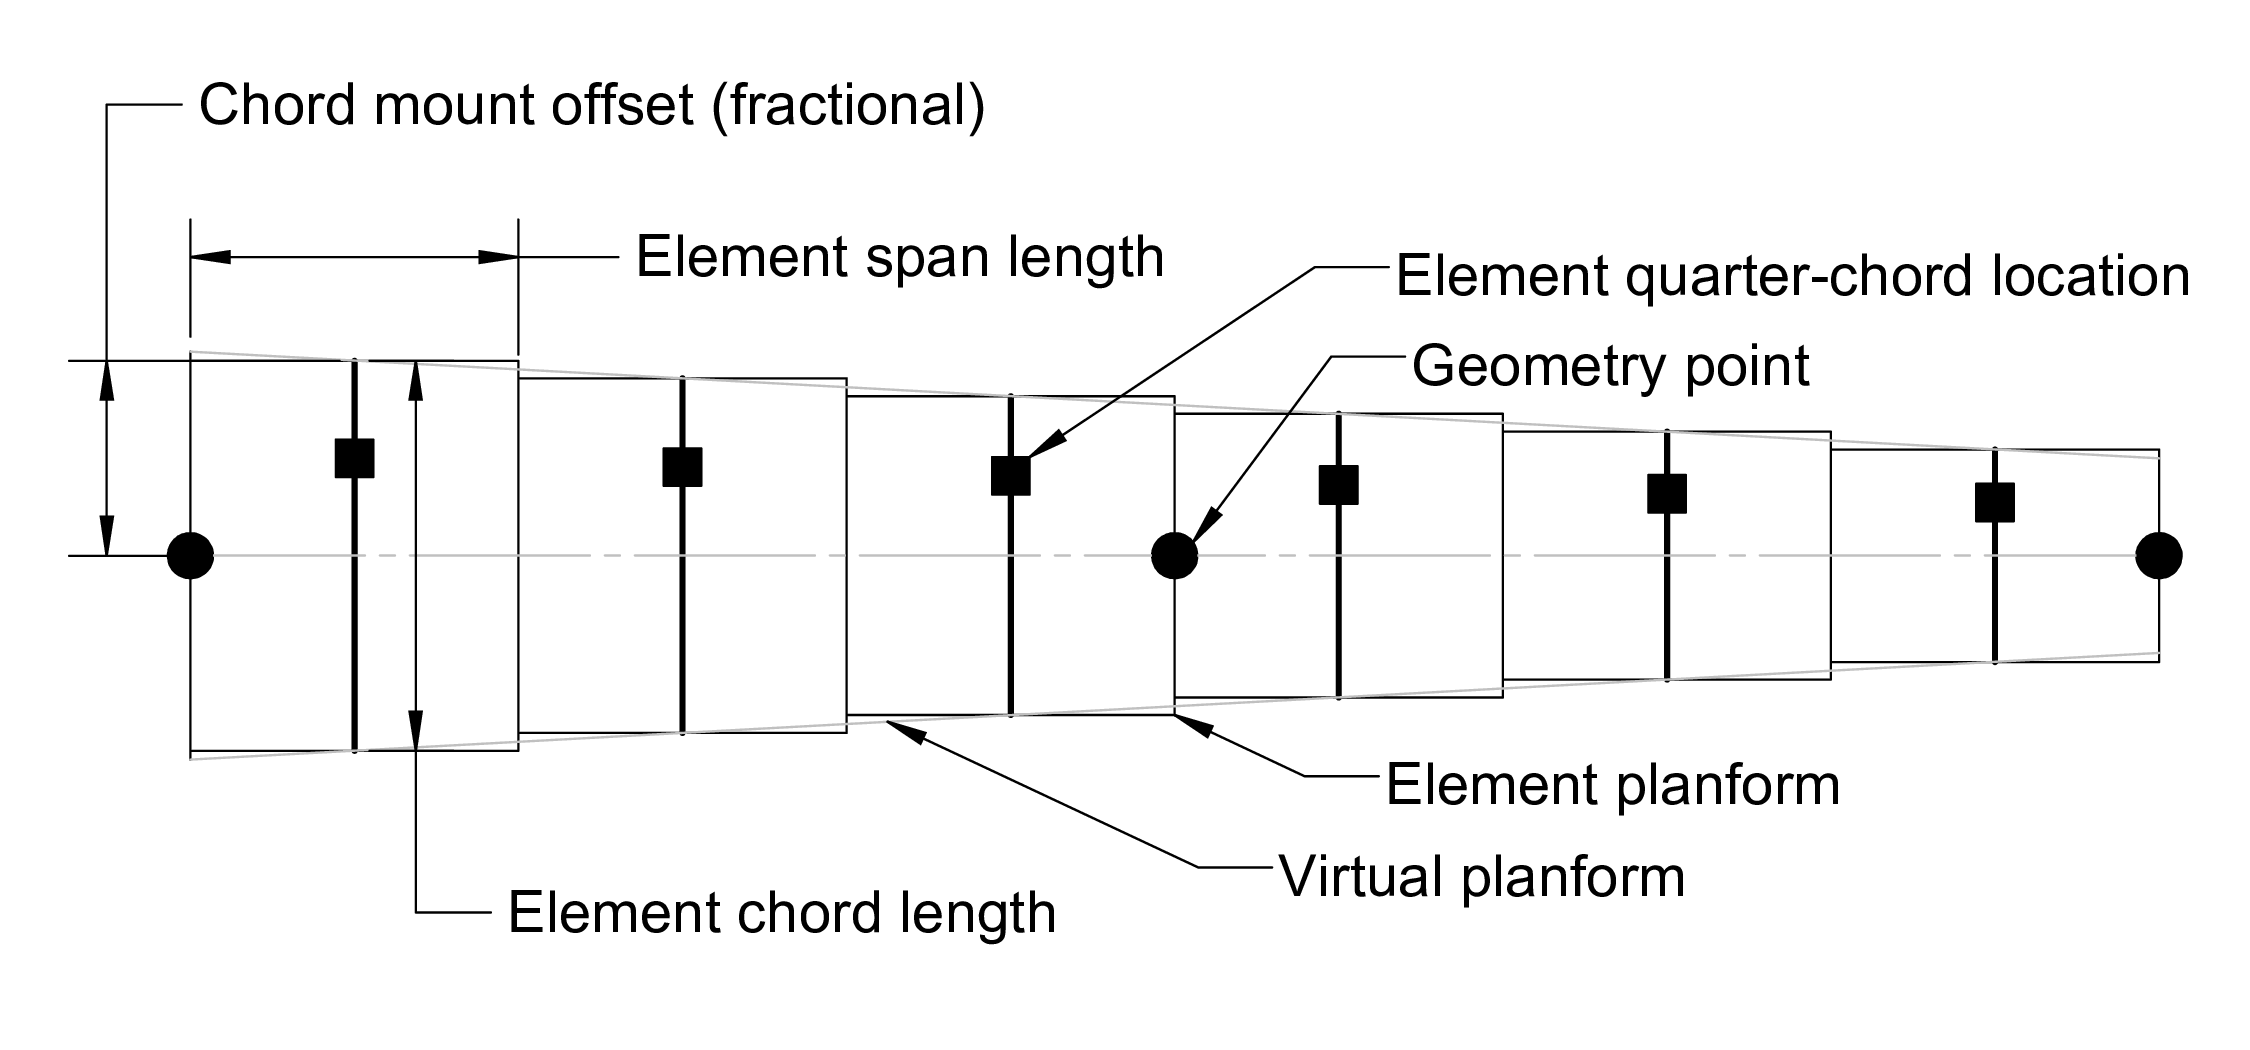
\includegraphics[width=0.9\textwidth]{alm-geometry}
    
    \caption{Actuator line geometry. Filled circles indicate geometry points
        whereas squares indicate actuator line element locations.}
    
    \label{fig:AL-geom}
\end{figure}


\section{Determining inflow velocity}

In momentum methods, the inflow velocity is determined by solving for the axial
and angular induction factors \cite{Manwell2002}. However, using Navier--Stokes
methods, it is somewhat unclear how to calculate the velocity vector used to
compute the angle of attack and relative velocity, though we have access to much
more information about the flow. Sorensen and Shen used an actuator line
element's position to determine the inflow velocity for an axial-flow turbine
\cite{Sorensen2002}. Similarly, Shamsoddin and Porte-Agel use the velocity at a
blade element's location in their actuator line simulation of a vertical-axis
turbine using LES \cite{Shamsoddin2014}. NREL's SOWFA ALM for OpenFOAM also uses
the velocity at the actuator line element location for computing inflow velocity
and local angle of attack with no corrections \cite{Churchfield2013}.

Schito and Zasso developed an effective velocity model (EVM) for computing
actuator forces in Navier--Stokes simulations \cite{Schito2014}. Their EVM
proposes that inflow velocity should be sampled along a line perpendicular to
the mean relative flow direction. They ultimately chose a the line to be 1.5
chord lengths upstream of the actuator point (i.e. quarter-chord location). A
sampling line was chosen to be 5 times the local mesh cell length. Finally, an
angle of attack correction is proposed
\begin{equation}
    \Delta \alpha = \frac{c}{M} (1.2553 - 0.0552 C_d) C_l,
    \label{eq:EVM-dalpha}
\end{equation}
where $c$ is the chord length, $M$ is the mesh size, and $C_l$ and $C_d$ are the
lift and drag coefficients, respectively. Note that the constants in
Equation~\ref{eq:EVM-dalpha} were determined from a calibration with 2-D
blade-resolved CFD for a NACA 0012 foil and are not assumed to be universal.

The EVM, despite showing robustness for its chosen validation case,
unfortunately involves determination of two unknown tuning parameters. To avoid
the additional effort and uncertainty in determining these, the inflow velocity
was sampled at the element quarter-chord location using OpenFOAM's
\texttt{interpolationCellPoint} class, which provides a linear weighted
interpolation using cell values. This algorithm helps keep the sampled velocity
``smooth'' compared with using the cell values themselves, especially when
elements are moving in space as they are in a turbine, since meshes will likely
have a cell size on the same order as the chord length, and will move on the
order of one cell length per time step.


\section{Static foil coefficient data}

Static input foil coefficient data were taken from Sheldahl and
Klimas~\cite{Sheldahl1981}---a popular database developed for CFTs, which
contains values over a wide range of Reynolds numbers. NACA 0021 coefficients
were used for both turbines, despite the fact that the UNH-RVAT is constructed
from NACA 0020 foils, as a NACA 0020 dataset is not available---it is assumed
the small difference in foil thickness is negligible. Since pitching moment data
were only available at limited Reynolds numbers, two datasets were used: The
lowest for $Re_c \leq 3.6 \times 10^5$ and highest $Re_c \geq 6.8 \times 10^5$.
For each actuator line element, blade chord Reynolds number is computed based on
the sampled inflow velocity, and the static coefficients are then interpolated
linearly within the database.


\section{Force projection}

After the force on the ALE from the flow is calculated, it is then projected
back onto the flow field as a source term in the momentum equation. To avoid
instability due to sharp gradients, the source term is tapered from its maximum
value away from the element location by means of a spherical Gaussian function.
The width of this function $\eta$ is controlled by a single parameter
$\epsilon$, which is then multiplied by the actuator line element force and
imparted on a cell with distance $| \vec{r} |$ from the actuator line element
quarter chord location:
\begin{equation}
    \eta = \frac{1}{\epsilon^3 \pi^{3/2}} \exp 
    \left[ - \left( \frac{| \vec{r} |}{\epsilon} \right)^2 \right].
    \label{eq:projection}
\end{equation}

Troldborg~\cite{Troldborg2008} proposed that the Gaussian width should be set to
twice the local cell length $\Delta x$ in order to maintain numerical stability.

Jha \emph{et al.}~\cite{Jha2014} provides guidelines for choosing a projection
width.

Schito and Zasso \cite{Schito2014} found that a projection $\epsilon$ equal to
the local mesh length was optimal.

Martinez-Tossas and Meneveau \cite{Martinez-Tossas2015b} used a 2-D potential
flow analysis to determine that the optimal projection width for a lifting
surface is 14--25\% of the chord length. The width due to the wake caused by the
foil drag force was recommended to be on the order of the momentum thickness
$\theta$, which for a bluff body or foil at large angle of attack is related to
the drag coefficient ($O(1)$) by \cite{TennekesAndLumley}
\begin{equation}
    C_d = 2 \theta / l,
    \label{eq:mom-thickness}
\end{equation}
where $l$ is a reference length, e.g., diameter for a cylinder or chord length
for a foil.

Using these guidelines, three Gaussian width values were determined: one
relative to the chord length, one to the mesh size, and one to the momentum
thickness due to drag force. Each three were computed for all elements at each
time step, and the largest was chosen for the force projection algorithm. Using
this adaptive strategy, fine meshes could benefit from the increased accuracy of
more concentrated momentum sources, and coarse meshes would be protected from
numerical instability.

The Gaussian width due to mesh size $\epsilon_{\mathrm{mesh}}$ was determined
locally on an element-wise basis by estimating the size of the cell containing
the element as
\begin{equation}
    \Delta x \approx \sqrt[3]{V_\mathrm{cell}},
\end{equation}
where $V_\mathrm{cell}$ is the cell volume. To account for the possibility of non-unity aspect ratio cells, an additional factor $C_\mathrm{mesh}$, 2.0 by default, was introduced, giving
\begin{equation}
    \epsilon_{\mathrm{mesh}} = 2C_\mathrm{mesh} \Delta x.
\end{equation}


\section{Unsteady effects}

In the context of a turbine---especially a cross-flow turbine---the actuator
lines will encounter unsteady conditions, both in their angle of attack and
relative velocity. These conditions necessitate the use of unsteady aerodynamic
models to augment the static foil characteristics, both to capture the time
resolved response of the attached flow loading and effects of flow acceleration,
also know as added mass. Furthermore, the angles of attack encountered by a CFT
blade will often be high enough to encounter dynamic stall (DS). It is therefore
necessary to model both unsteady attached and detached flow to obtain accurate
loading predictions.


\subsection{Dynamic stall}

Dynamic stall is encountered when the blade angle of attack changes rapidly in
time and exceeds a certain threshold, often near the static stall angle
\cite{McCroskey1981}. The stall is characterized by an initial increase in lift
beyond static values as a vortex is shed from the foil's leading edge, after
which a drop in lift and large nose-down pitching moment occurs as the vortex is
advected downstream. As the angle of attack drops below the critical value, flow
reattaches, closing the so-called hysteresis loop. Dynamic stall has been shown
to be a significant positive contributor to performance in CFTs \cite{Para2002,
    Urbina2013}, therefore an accurate model is key.

\todo[inline]{Add figure showing dynamic stall cycle.}

DS models were first developed to improve predictive capability for helicopter
rotors, on which DS has significant effects on maneuverability and operational
envelope \cite{Bousman2000}. A summary of dynamic stall models developed for
helicopter rotors is presented in \cite{Leishman2006}. The simplest dynamic
stall models rely on semi-empirical correlations, e.g., the Gormont model
\cite{Gormont1973}, developed at the Boeing--Vertol Company. Several variants of
the Gormont model were developed for vertical-axis wind turbines, with varying
degrees of success; a summary is presented in \cite{Para2002}.

Leishman and Beddoes (LB) developed a semi-empirical model for unsteady
aerodynamics and dynamic stall, which is derived from the phenomenology of the
physics instead rather than pure empiricism \cite{Leishman1989}. Beddoes then
updated the model to the so-called third generation or ``3G'' version
\cite{Beddoes1993}. The LB DS models can be summarized conceptually based on the
following principles:
\begin{itemize}
    \item Dynamic conditions cause a time lag in effective angle of attack and
    lift force.
    
    \item Separation is determined by the Kirchoff flow approximation, which is
    also used to parameterize the normal force coefficient table based on the
    trailing edge separation point. This separation point also encounters a time
    lag.
    
    \item The separation initiates a vortex shedding cycle that causes an
    overshoot and subsequent undershoot in lift before returning to an attached
    flow condition.
\end{itemize}

Sheng et al. \cite{Sheng2008} developed an LB DS model variant targeted at low
Mach numbers. This model, along with the original and 3G LB DS model variants,
was tested for its effectiveness in cross-flow turbine conditions by Dyachuk et
al.~\cite{Dyachuk2014}, who concluded that the Sheng et al. variant results
matched most closely with experiments. In a similar study, the Sheng et al.
model also faired better than the Gormont model \cite{Dyachuk2015}, which
inspired its adoption here for the ALM.

Before the dynamic stall subroutine is executed, the static profile data for
each element is interpolated linearly based on local chord Reynolds number. The
profile data characteristics---static stall angle, zero-lift drag coefficient,
and separation point curve fit parameters---are then recomputed each time step
such that the effects of Reynolds number on the static data are included.

Inside the ALM, angle of attack is sampled from the flow field rather than
calculated based on the geometric angle of attack. Therefore, the implementation
of the LB DS model was such that the equivalent angle of attack
$\alpha_\mathrm{equiv}$ was taken as the sampled rather than the lagged
geometric value. A similar implementation was used by Dyachuk et al.
\cite{Dyachuk2015a} inside a vortex model.


\subsection{Added mass}

A correction for added mass effects, or the effects due to accelerating the
fluid, was taken from Strickland \emph{et al.}~\cite{Strickland1981}, which was
derived by considering a pitching flat plate in potential flow. In the blade
element coordinate system, the normal and chordwise (pointing from trailing to
leading edge, which is opposite the $x$-direction used by Strickland \emph{et
    al.}) coefficients due to added mass are
\begin{equation}
    C_{n_\mathrm{AM}} = -\frac{\pi c \dot{U_n}}{8 | U_\mathrm{rel} |^2}, 
\end{equation}
and
\begin{equation}
    C_{c_\mathrm{AM}} = \frac{\pi c \dot{\alpha} U_n }{8 | U_\mathrm{rel} |^2}, 
\end{equation}
respectively, where $U_n$ is the normal component of the relative velocity, and
dotted variables indicate time derivatives, which were calculated using a simple
first order backward finite difference. Similarly, the quarter-chord moment
coefficient due to added mass was calculated as
\begin{equation}
    C_{m_\mathrm{AM}} = -\frac{C_{n_\mathrm{AM}}}{4} 
        - \frac{U_n U_c}{8 | U_\mathrm{rel} |^2},
\end{equation}
where $U_c$ is the chordwise component of relative velocity. Note that the
direction of positive moment is ``nose-up,'' which is opposite that used by
Strickland \emph{et al.}.

The normal and chordwise added mass coefficients translate to lift and drag
coefficients by
\begin{equation}
    C_{l_\mathrm{AM}} = C_{n_\mathrm{AM}} \cos \alpha + C_{c_\mathrm{AM}} \sin
    \alpha,
\end{equation}
and
\begin{equation}
    C_{d_\mathrm{AM}} = C_{n_\mathrm{AM}} \sin \alpha - C_{c_\mathrm{AM}} \cos
    \alpha,
\end{equation}
respectively. The added mass coefficients were then added to those calculated by
the dynamic stall model.


\section{Flow curvature corrections}

The rotating blades of a cross-flow turbine will have varying angle of attack
along their chords for any given azimuthal location due to the circular
path---producing so-called flow curvature effects~\cite{Migliore1980}. This
makes it difficult to define a single angle of attack for use in the static
coefficient lookup tables. Furthermore, this effect is more pronounced for high
solidity ($c/R$) turbines. Two different flow curvature corrections were
considered; one by Goude \cite{Goude2012} and one by Mandal and Burton
\cite{Mandal1994}.

The Goude correction is derived by considering a flat plat moving along a
circular path in potential flow.

\begin{equation}
    \alpha = \delta + \arctan \frac{V_\mathrm{abs} \cos(\theta_b -
        \beta)}{V_\mathrm{abs} \sin(\theta_b - \beta) + \Omega R} - \frac{\Omega
        x_{0r}c}{V_\mathrm{ref}} - \frac{\Omega c}{4 V_\mathrm{ref}},
    \label{eq:Goude-curvature}
\end{equation}
where $\delta$ is the blade pitch angle, $V_\mathrm{abs}$ is the magnitude of
the local inflow velocity at the blade, $\theta_b$ is the blade azimuthal
position, $\beta$ is the direction of the inflow velocity, $\Omega$ is the
turbine's angular velocity, $R$ is the blade element radius, $x_{0r}$ is a
normalized blade attachment point along the chord, $c$ is the blade chord
length, and $V_\mathrm{ref}$ is the reference flow velocity for calculating
angle of attack.

Note that the code uses vector objects and their associated arithmetic in
software (thanks to OpenFOAM's \texttt{vector} class), which means the first two
terms in Equation~\ref{eq:Goude-curvature} are taken care of automatically given
the inflow velocity, chord direction, and element velocity vectors. Therefore,
the last two terms in Equation~\ref{eq:Goude-curvature} was simply added to the
scalar angle of attack. Note that for a cross-flow turbine, this correction
effectively offsets the angle of attack, which therefore increases its magnitude
on the upstream half of the blade path, and decreases its magnitude on the
downstream half, where the angle of attack is negative.

The Mandal--Burton flow curvature correction assumes that since the blade is
encountering a curvilinear flow, it can be treated as having virtual camber.
They introduce a factor to describe the variation of angle of attack from the
leading to trailing edge
\begin{equation}
    \Delta \alpha = \alpha_\mathrm{TE} - \alpha_\mathrm{LE},
    \label{eq:Mandal-Burton-alpha-diff}
\end{equation}
where TE and LE subscripts denote the values of angle of attack at the trailing
and leading edge, respectively. Calculating these values for an actuator line
element can be done by tracking the leading and trailing edge locations and
velocities, then performing the same vector arithmetic used to calculate the
quarter-chord angle of attack.

An incidence correction factor
\begin{equation}
    \alpha_c = \arctan \left( \frac{1 - \cos (\Delta \alpha / 2)}{\sin (\Delta
        \alpha / 2)} \right)
    \label{eq:Mandal-Burton-alpha-corr}
\end{equation}
is introduced and added to the uncorrected angle of attack. Like the Goude
model, $\alpha_c$ is positive on the upstream half of the turbine rotation and
negative on the downstream half. Both implementations are shown in
Listing~\ref{lst:flow-curvature}.

\begin{lstlisting}[float,caption=Flow curvature model implementation.,label=lst:flow-curvature]
    if (flowCurvatureModelName_ == "Goude")
    {
        angleOfAttackRad += omega_*(chordMount_ - 0.25)
                         * chordLength_/mag(relativeVelocity_);
        angleOfAttackRad += omega_*chordLength_/(4*mag(relativeVelocity_));
    }
    else if (flowCurvatureModelName_ == "MandalBurton")
    {
        // Calculate relative velocity at leading and trailing edge
        vector relativeVelocityLE = inflowVelocity_ - velocityLE_;
        vector relativeVelocityTE = inflowVelocity_ - velocityTE_;
    
        // Calculate vector normal to chord--span plane
        vector planformNormal = -chordDirection_ ^ spanDirection_;
        planformNormal /= mag(planformNormal);
        
        // Calculate angle of attack at leading and trailing edge
        scalar alphaLE = asin((planformNormal & relativeVelocityLE)
                       / (mag(planformNormal)*mag(relativeVelocityLE)));
        scalar alphaTE = asin((planformNormal & relativeVelocityTE)
                       / (mag(planformNormal)*mag(relativeVelocityTE)));
        
        scalar beta = alphaTE - alphaLE;
        
        angleOfAttackRad += atan2((1.0 - cos(beta/2.0)), sin(beta/2.0));
    }
\end{lstlisting}


\section{End effects}

Helmholtz's second vortex theorem states that vortex lines may not end in a
fluid, but must either form closed loops or extend to boundaries. Consequently
the lift distribution due to the bound vortex from foils of finite span must
drop to zero at the tips.

Glauert used Prandtl's lifting line theory to develop a tip loss correction
factor for the blade element analysis of an axial-flow rotor. This was further
developed for horizontal-axis wind turbines by Shen et al. \cite{Shen2005a}.
However, these corrections both depend on the axial-flow rotor tip speed ratio,
number of blades, and tip flow angle, which do not necessarily directly
correspond to cross-flow rotor parameters. Therefore, a more general end effects
model was sought.

From Prandtl's lifting line theory, the geometric angle of attack $\alpha$ of a
foil with an arbitrary circulation distribution can be expressed as a function
of nondimensional span $\theta$ as \cite{Anderson2001}
\begin{equation}
    \alpha (\theta) = \frac{2S}{\pi c (\theta)}
    \sum_1^N A_n \sin \theta
    + \sum_1^N n A_n \frac{\sin n \theta}{\sin \theta}
    + \alpha_{L = 0}(\theta),
    \label{eq:lifting-line}
\end{equation}
where $S$ is the span length, $c(\theta)$ is the chord length, and $N$ is the
number of locations or elements sampled along the foil. This relationship can be
rearranged into a matrix equation to solve for the unknown Fourier coefficients
$A_n$,
\begin{equation}
    [\alpha_m ] - \alpha_{L=0} = [D_{mn}][A_n],
\end{equation}
where
\begin{equation}
    D_{mn} = \sum_1^N \left[ \frac{2b}{\pi c_m} \sin n \theta_m + n \frac{\sin n
        \theta_m}{\sin \theta_m} \right].
\end{equation}

With the Fourier coefficients, the circulation distribution can be calculated as
\begin{equation}
    \Gamma (\theta) = 2SU_\infty \sum_1^N A_n \sin n \theta,
\end{equation}
which, via the Kutta--Joukowski theorem, provides the lift coefficient
distribution
\begin{equation}
    C_l(\theta) = \frac{-\Gamma (\theta)}{\frac{1}{2} c U_\infty}.
\end{equation}

We can therefore compute a correction function 
\begin{equation}
    F = C_l(\theta)/C_l(\theta)_{\max},
\end{equation}
which will be in the range $[0, 1]$, similar to the Glauert corrections, but
does not contain rotor parameters. The correction function for various methods
is compared in Figure~\ref{fig:end-effects}.

\begin{figure}
    \centering
    
    \caption{End effect correction function values for the Glauert, Shen et al.,
        and lifting line methods.}
    
    \label{fig:end-effects}
\end{figure}


\section{Software implementation}

The USA National Renewable Energy Laboratory (NREL) has developed and released
an actuator line modeling library, SOFWA~\cite{Churchfield2014b}, for simulating
horizontal-axis wind turbine arrays using the OpenFOAM finite volume CFD
library. OpenFOAM is free, open-source, and widely used throughout industry and
academia. Though SOWFA is also open-source, its procedural style would have
required significant effort and duplicate code to adapt for cross-flow turbines.
Thus, a new and more general ALM library was developed from the ground up that
could model both cross- and axial-flow turbines, as well as standalone actuator
lines. The actuator line model developed here, dubbed \textit{turbinesFoam}, was
also written as an extension library for OpenFOAM, and was developed freely and
openly from the start in order to increase community engagement and research
efficiency.

\textit{turbinesFoam} was written in OpenFOAM's style, using OpenFOAM's
\texttt{fvOptions} framework for adding source terms to equations at
runtime---see Listing~\ref{lst:fvOptions} for an example implementation within
the Navier--Stokes' momentum equation. Using the \texttt{fvOptions} framework
allows the CFT-ALM to be added to many of the solvers included in OpenFOAM,
meaning it can be readily used with RANS or LES, multiphase models (e.g., for
simulating the free surface in MHK installations), and even with heat transfer.
This is in contrast to SOWFA's implementation, which requires custom flow
solvers to be developed and maintained.

\begin{lstlisting}[float,caption=Adding source terms to the momentum equation in OpenFOAM.,label=lst:fvOptions]
    tmp<fvVectorMatrix> UEqn
    (
        fvm::ddt(U)
        + fvm::div(phi, U)
        + turbulence->divDevReff(U)
        ==
        fvOptions(U)
    );
\end{lstlisting}

OpenFOAM and \textit{turbinesFoam} are written in the C++ programming language,
which follows the object oriented programming paradigm. This characteristic
helped modularize the ALM code for increased readability and reuse. In
\textit{turbinesFoam}, a turbine is a software object that is composed of
actuator line objects, which themselves are composed of actuator line element
objects. Structuring the code this way allows isolation and reuse of the
functionality of individual components. For example, the actuator line object
was written such that is could be used outside the turbine context to ensure is
produces the correct forcing, without adding the complexity of rotation, other
actuator lines, etc. that would be present in a turbine rotor. The very same
actuator line objects can be used in both axial-flow and cross-flow rotors,
without having to copy code from one to the other. In contrast, the actuator
line model in \textit{SOWFA} uses a single software object to represent an
entire array of turbines, which necessitates iterating through many nested lists
down to the element level, which can be confusing to read.

OpenFOAM's data structures are designed to be inherently parallel via message
passing interface (MPI). By working within the library infrastructure the ALM
code was easily parallelized, which will facilitate its deployment on high
performance computing clusters for large flow simulations.

Since all applications are run from a command line and all input data is text
based, automation and integration with other tools is relatively
straightforward. Future enhancements could include coupling with software for
generating static foil data, e.g., XFOIL or other OpenFOAM solvers, turbine
controller models, structural analysis codes, and optimization tools, e.g.,
SNL's DAKOTA \todo[inline]{Get citation for DAKOTA.}, for both individual
turbines and array layouts.


\section{Results}

Both the high solidity UNH-RVAT and low to medium solidity RM2 turbines were
simulated using a $k$--$\epsilon$ Reynolds-averaged Navier--Stokes (RANS)
turbulence model. These rotors provide diverse parameters, which helped evaluate
the robustness of the ALM. The simulations were performed inside a domain
similar in size to that used in Chapter~\ref{chap:CFD}, with similar boundary
conditions. A slice of the mesh in the $x$--$y$ plane is shown in
Figure~\ref{fig:ALM-mesh}.

\begin{figure}
    
    \caption{$x$--$y$ planar slice of the mesh used for the ALM RANS
        simulations.}
    
    \label{fig:ALM-mesh}
\end{figure}

Similar numerical settings were used for each turbine as well. The Sheng et al.
DS model was used with the default coefficients given in \cite{Sheng2008}, and
the Goude flow curvature correction was employed. A second order backward
difference was used for advancing the simulation in time, and second order
linear schemes were used for the majority of the terms' spatial discretizations.
The only major difference between the two simulation configurations was that the
end effects model was deactivated for the RM2, since it reduced $C_P$ far below
the experimental measurements. This modification is at least consistent with the
RM2 blades' higher aspect ratio and tapered planform. Case files for the
UNH-RVAT and RM2 ALM simulations are available from XXX and XXX, respectively.
\todo[inline]{Cite ALM case files.}

The same foil coefficient data were used for all simulations---those for a NACA
0021 as reported by Sheldahl and Klimas \cite{Sheldahl1981}. Each rotor's shaft
was assumed to have a drag coefficient $C_d = 1.1$, and the blade support strut
end element drag coefficients were set to 0.05, to approximate the effects of
separation in the corners of the blade--strut connections.

Since the ALM is intended to be an engineering tool when coupled with RANS, it
was assumed that information about tip speed ratio due to control details would
not be known a priori, and was excluded, unlike the 3-D blade-resolved cases in
Chapter~\ref{chap:CFD}. Note that a systematic investigation of the effects of
sinusoidal $\lambda$ was not undertaken, but for the UNH-RVAT a one to two
percentage point increase in $C_P$ was observed when running with similar
parameters as the blade-resolved simulation.

To evaluate the ALM's ability to predict wake characteristics in a high fidelity
simulation, the UNH-RVAT was also modeled using the Smagorinsky large-eddy
simulation (LES) turbulence model \cite{Smagorinsky1963} in a domain that was
extended slightly to allow for further wake development. Spatial and temporal
grid resolution modifications are discussed below.


\subsection{Verification}

Verification for sensitivity to spatial and temporal grid resolution was
performed for both the UNH-RVAT and RM2 RANS cases, the results from which are
plotted in Figure~\ref{fig:RVAT-ALM-verification} and
Figure~\ref{fig:RM2-ALM-verification}, respectively. Both models displayed low
sensitivity to the number of time steps per revolution. Spatial grid dependence,
however, was more dramatic.

\todo[inline]{Make quantitative statements about verification studies.}

\begin{figure}
    \centering
    
    \caption{Temporal (left) and spatial (right) grid resolution sensitivity
        results for the UNH-RVAT ALM RANS model.}
    
    \label{fig:RVAT-ALM-verification}
\end{figure}

\begin{figure}
    \centering
    
    \caption{Temporal (left) and spatial (right) grid resolution sensitivity
        results for the RM2 ALM RANS model.}
    
    \label{fig:RM2-ALM-verification}
\end{figure}


\subsection{UNH-RVAT RANS}

Power and drag coefficient curves are plotted for the UNH-RVAT in
Figure~\ref{fig:RVAT-ALM-perf-curves}. The ALM was successful at predicting the
performance tip speed ratios up to $\lambda_0$, which suggests that dynamic
stall was being modeled accurately, but $C_P$ was overpredicted at high
$\lambda$. This may have been caused by the omission of additional parasitic
drag sources such as exposed bolt heads and other imperfections located far
enough from the axis to have a large effect at high rotation rates. In
Chapter~\ref{chap:RM2} we showed how these losses can be significant even with
carefully smoothed struts and strut-blade connections. Overprediction of
performance at high tip speed ratio could also be a consequence of the
Leishman--Beddoes dynamic stall model, which can also be seen in the Darrieus
VAWT momentum model results shown in Figure 6.70 of \cite{Para2002}.

\begin{figure}
    \centering
    
    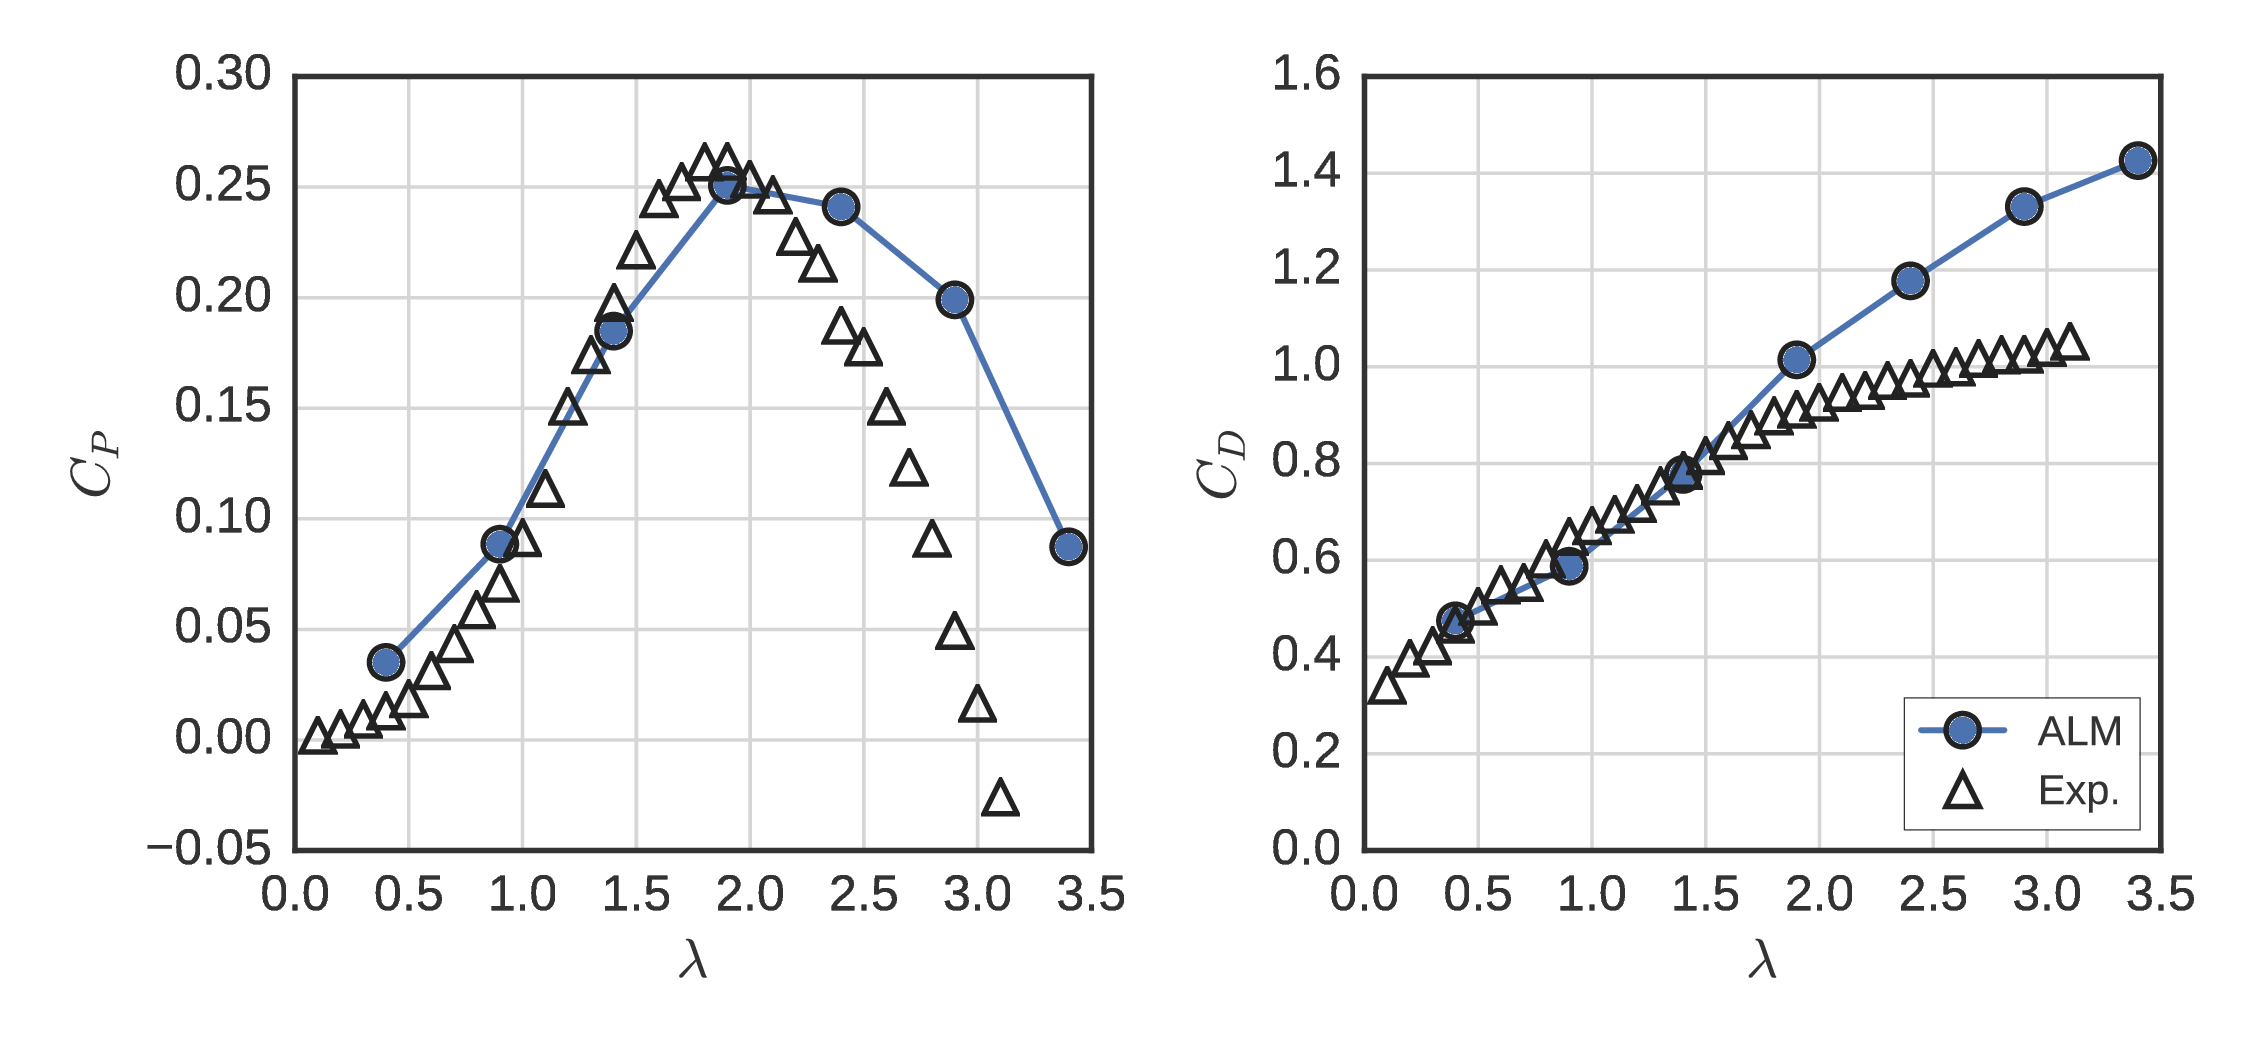
\includegraphics[width=0.85\textwidth]{RVAT-ALM_perf-curves}
    
    \caption{Power and drag coefficient curves computed for the UNH-RVAT using
        the actuator line model with RANS.}
    
    \label{fig:RVAT-ALM-perf-curves}
\end{figure}

Figure~\ref{fig:RVAT-ALM-meancontquiv} shows mean velocity field for the
UNH-RVAT computed by the ALM RANS model. The assymetry was captured well, along
with some of the vertical flow due to blade tip vortex shedding, though the flow
structure is missing the detail present in the experiments and blade-resolved
RANS simulations. Overall, the wake appears to be over-diffused, which could be
a consequence of the relatively coarse mesh. Note that with the DS and flow
curvature corrections turned off, the direction of the mean swirling motion
reverses, which highlights the importance of resolving the correct azimuthal
location of blade loading.

\begin{figure}
    \centering

    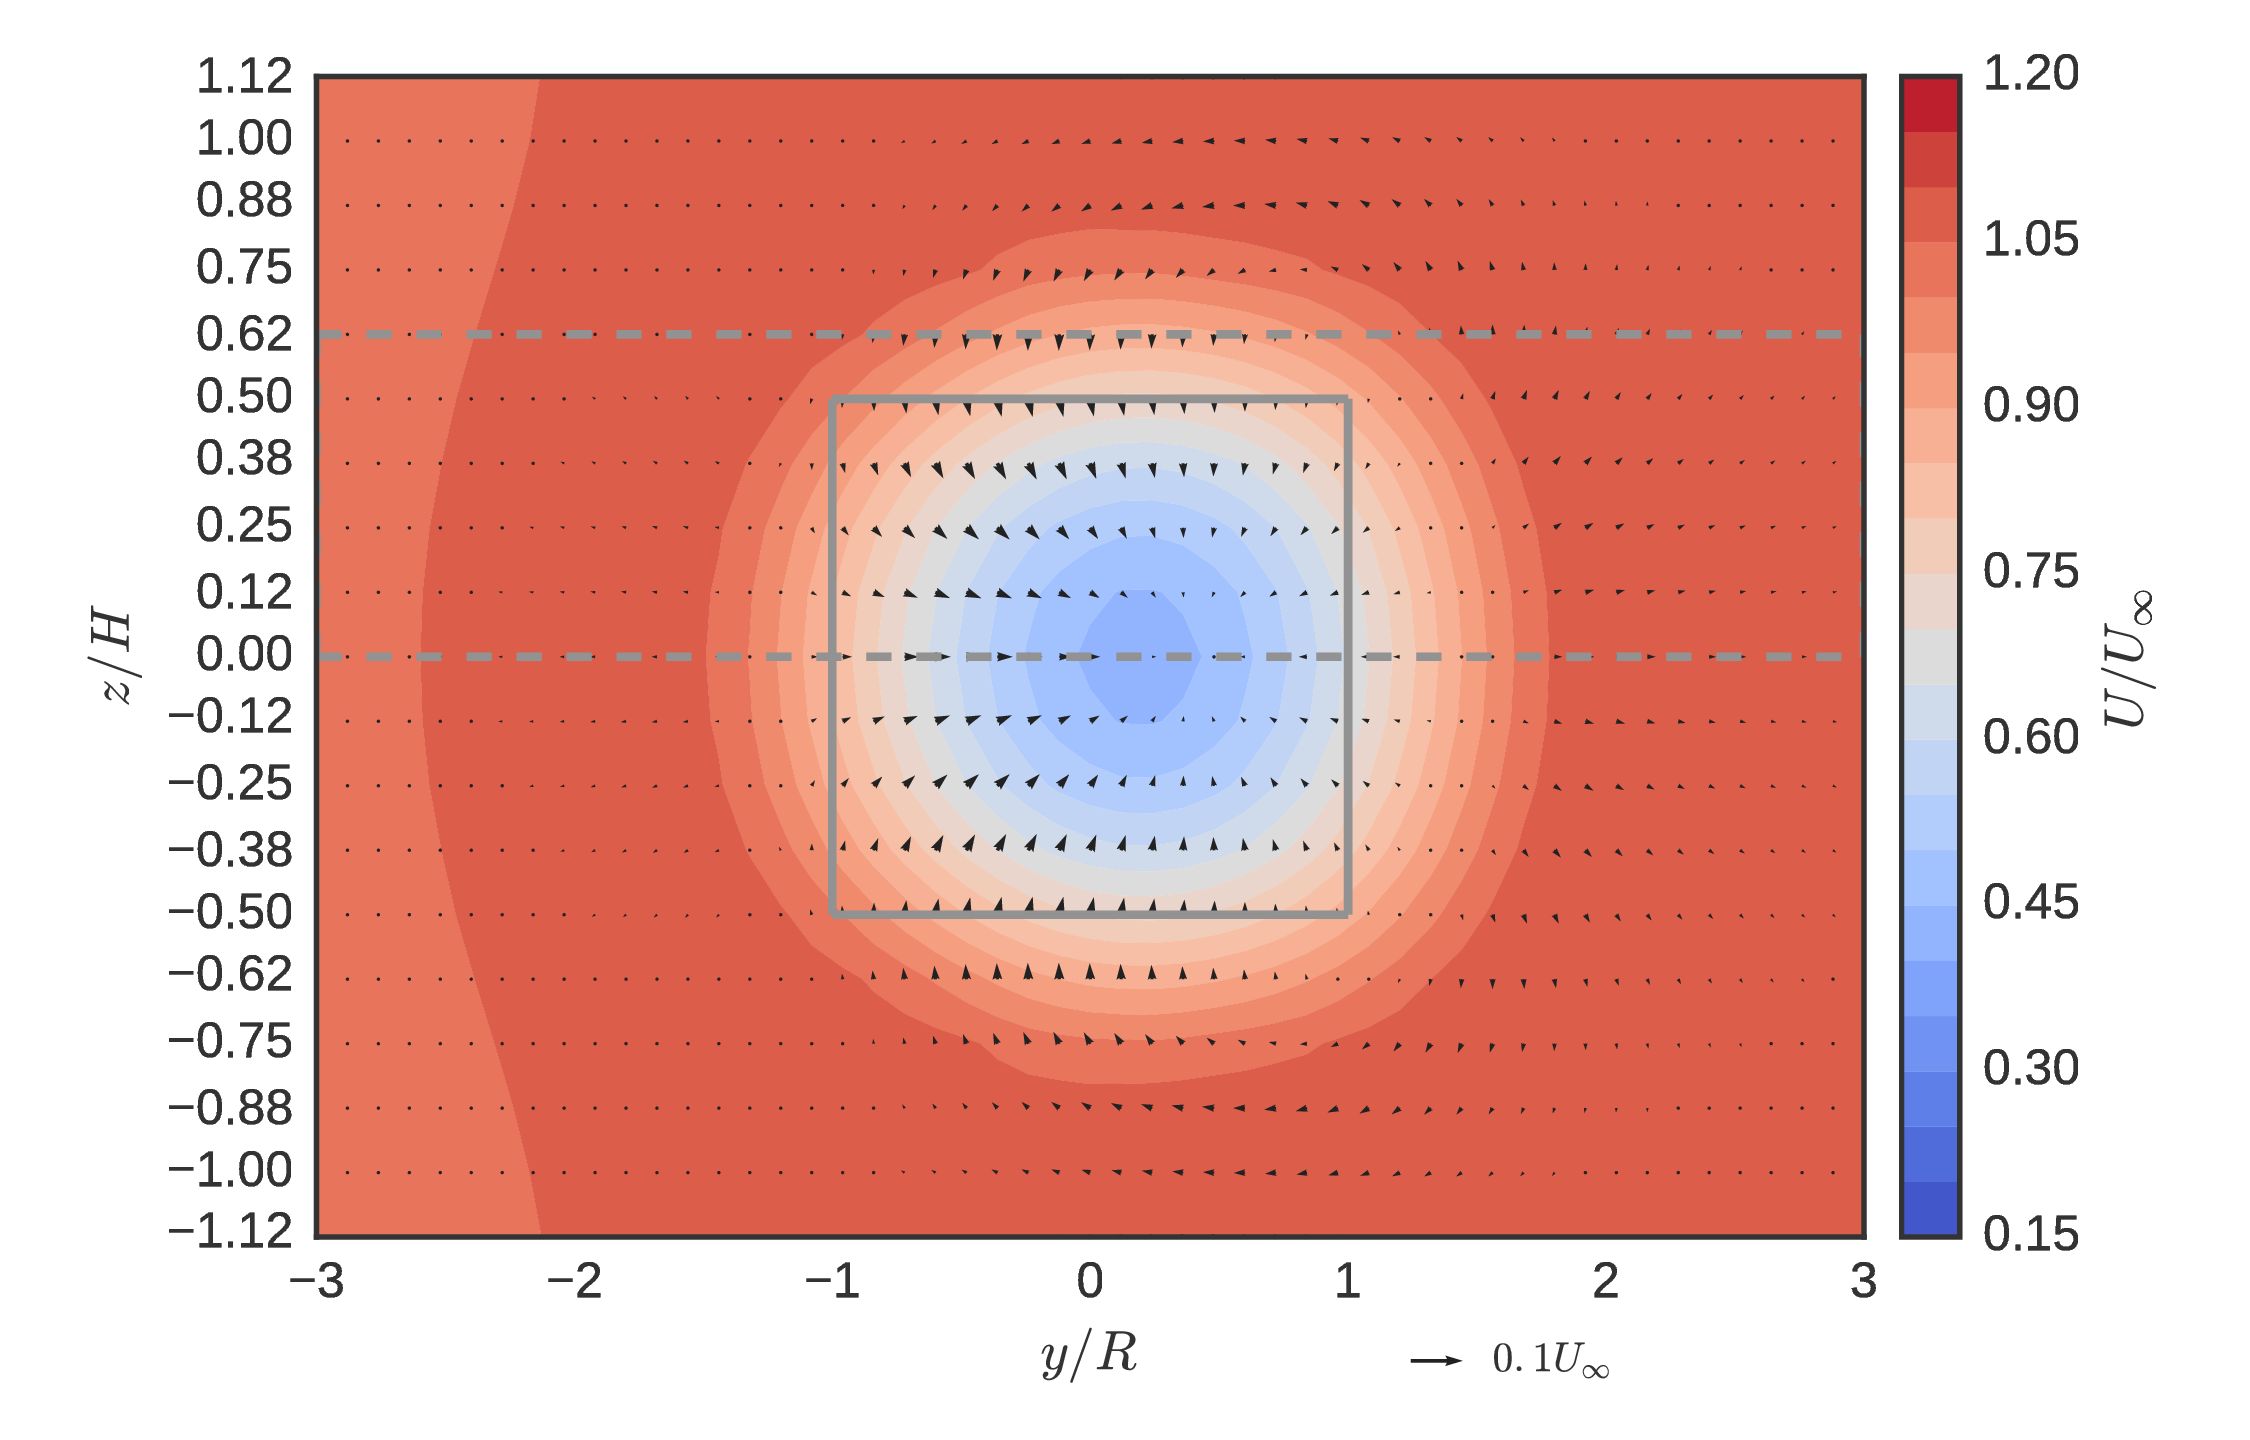
\includegraphics[width=0.9\textwidth]{RVAT-ALM_meancontquiv}
    
    \caption{Mean velocity field at $x/D=1$ with the LB-SGC model, with and
        without the Goude flow curvature correction.}
    
    \label{fig:RVAT-ALM-meancontquiv}
\end{figure}

Turbulence kinetic energy contours (including resolved and modeled energy) are
shown in Figure~\ref{fig:RVAT-ALM-kcont}. The ALM was able to resolve the
concentrated area of $k$ on the $+y$ side of the turbine, but the turbulence
generated by the dynamic stall vortex shedding process is absent. This makes
sense since in the ALM, the DS model only modulates the body force term in the
momentum equation, which does not provide a mechanism for mimicking shed
vortices or turbulence.

\begin{figure}
    \centering

    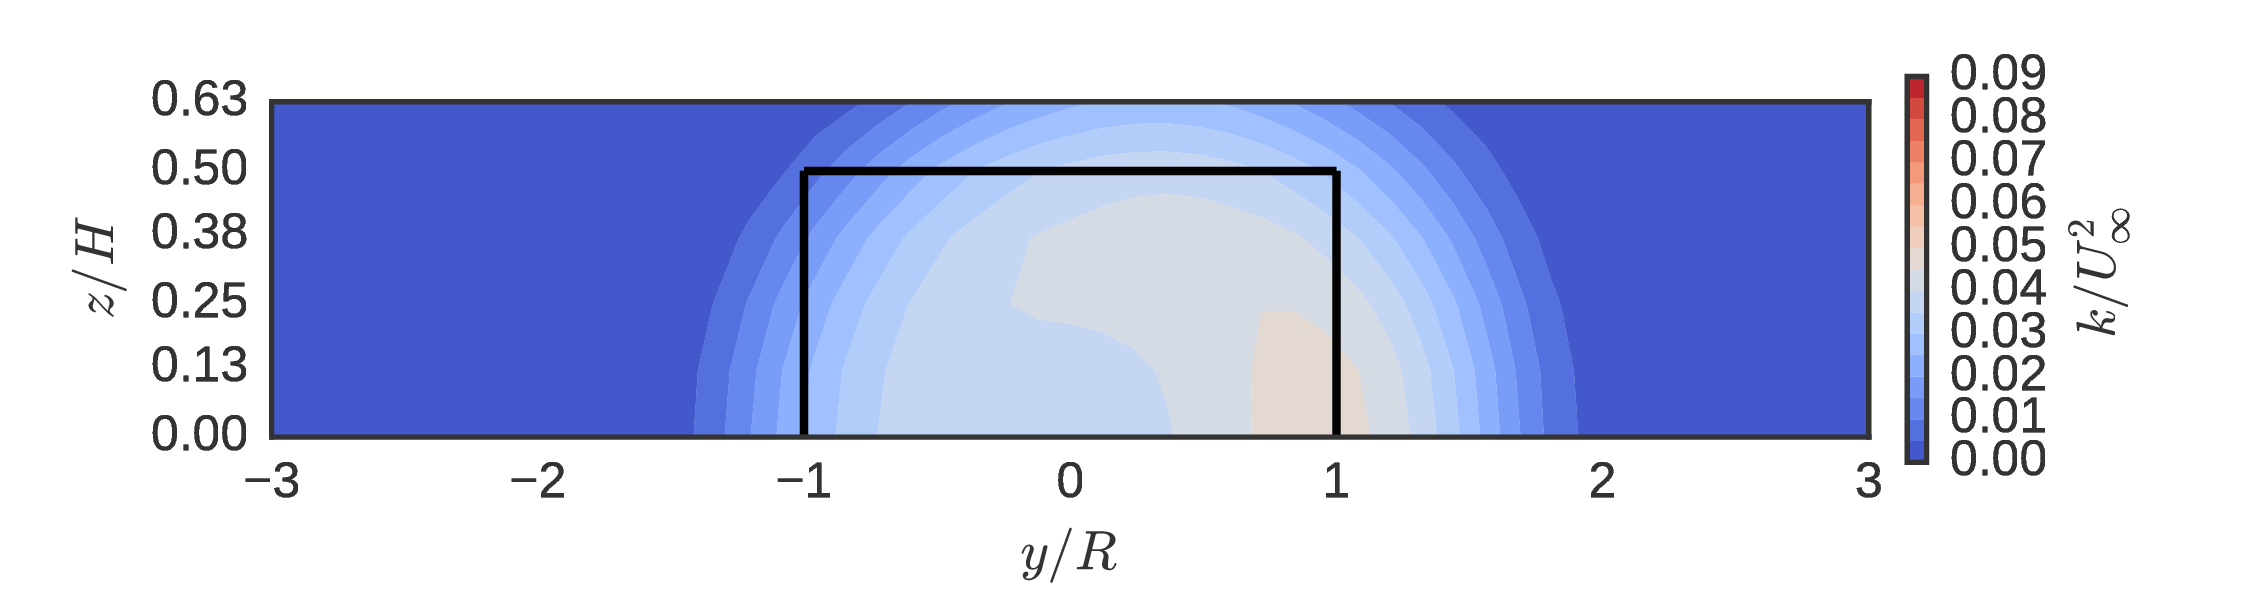
\includegraphics[width=0.85\textwidth]{RVAT-ALM_kcont}
    
    \caption{Turbulence kinetic energy contours at $x/D=1$ predicted by the
        ALM.}
    
    \label{fig:RVAT-ALM-kcont}
\end{figure}

Profiles of mean streamwise velocity and turbulence kinetic energy are shown in
Figure~\ref{fig:RVAT-ALM-profiles}. Here the over-diffused or over-recovered
characteristic of the mean velocity deficit seen in
Figure~\ref{fig:RVAT-ALM-meancontquiv} is more apparent. This effect is also
seen in the profile of $k$, where energy is smeared over the center region of
the rotor.

\begin{figure}
    \centering
    
    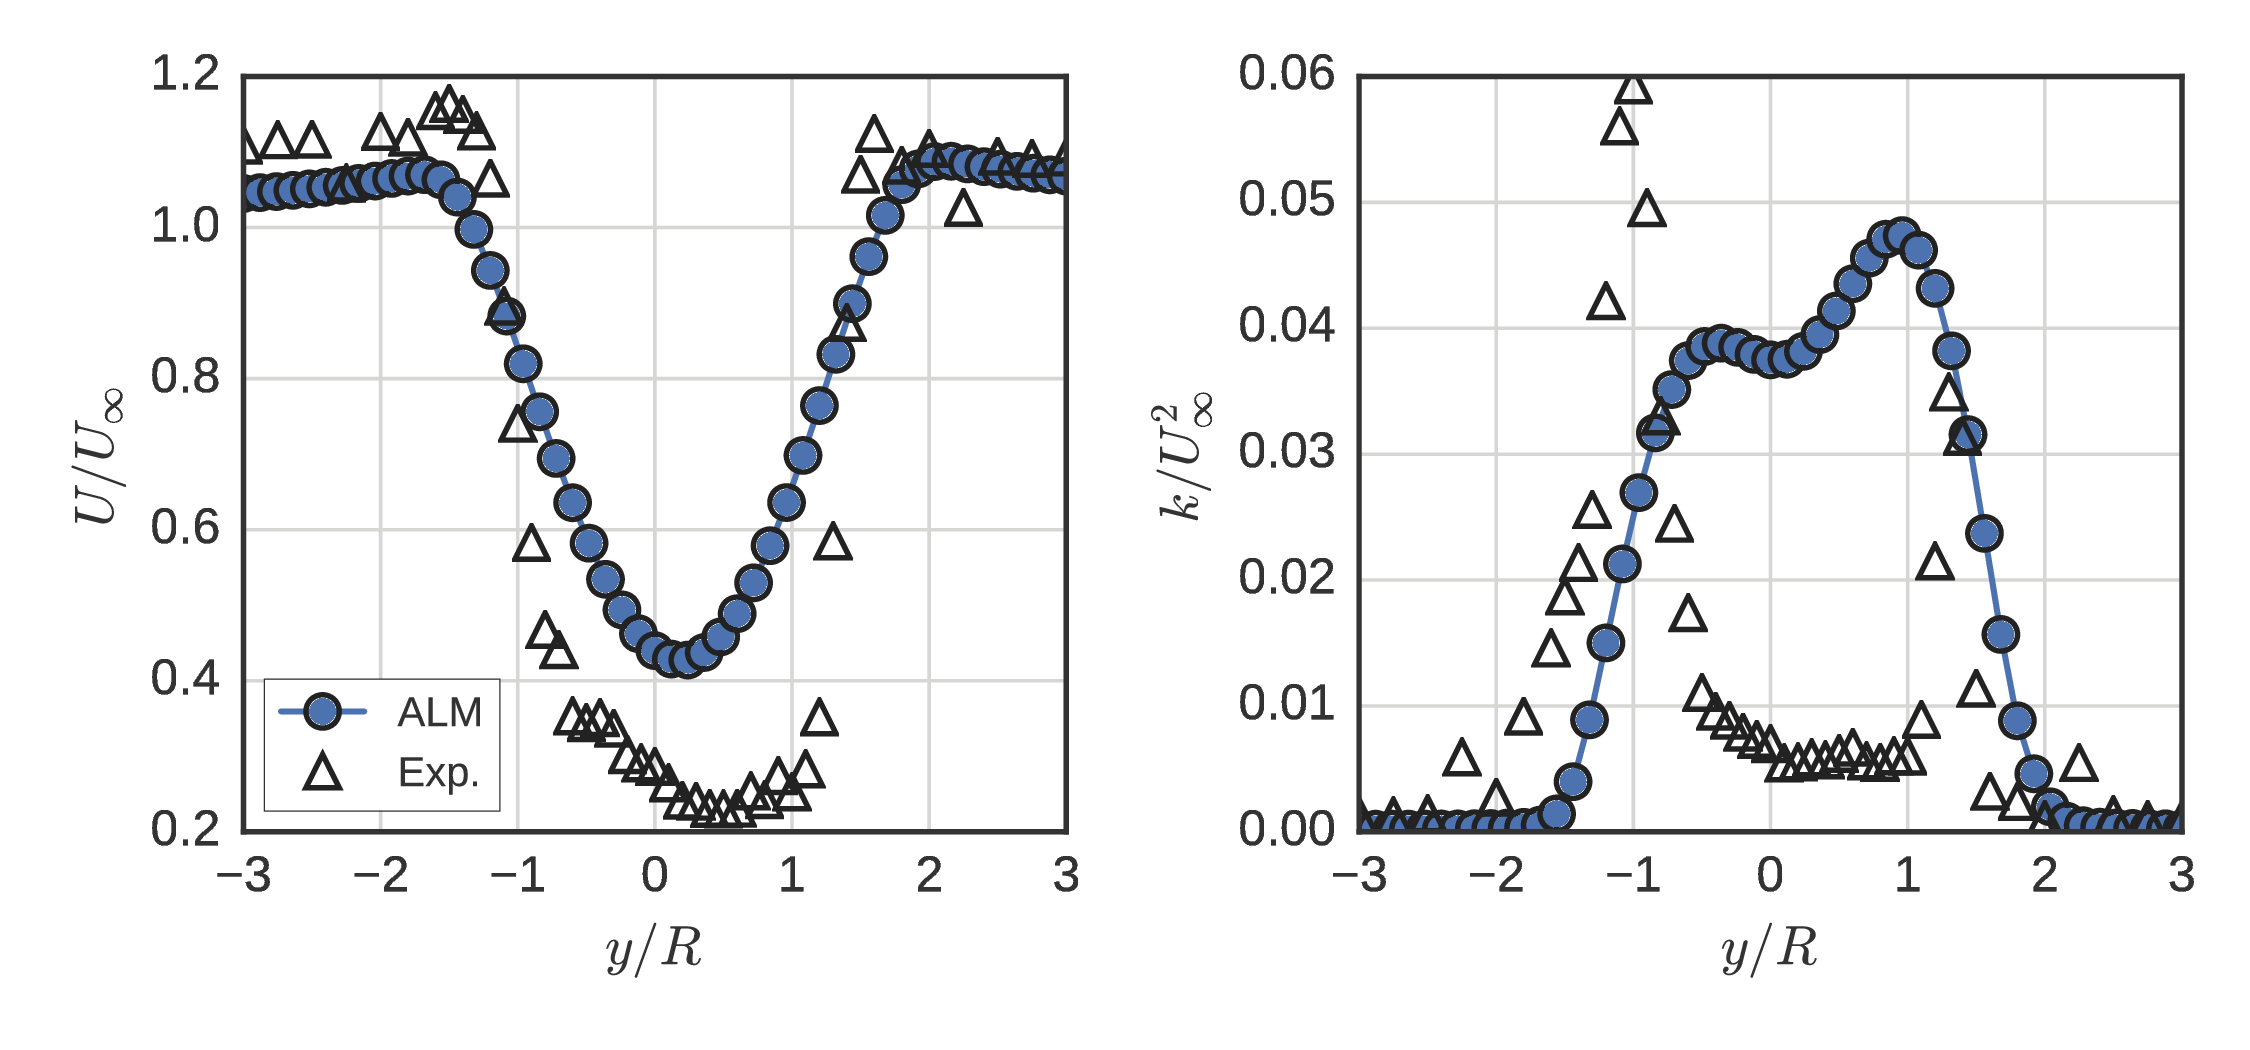
\includegraphics[width=0.85\textwidth]{RVAT-ALM_wake-profiles}
    
    \caption{Mean streamwise velocity (left) and turbulence kinetic energy
        (right) profiles at $z/H=0$ for the UNH-RVAT ALM.}
    
    \label{fig:RVAT-ALM-profiles}
\end{figure}

Weighted averages for the momentum recovery terms were computed identically as
they were in Chapter~\ref{chap:CFD}, and are plotted in
Figure~\ref{fig:RVAT-ALM-recovery} along with the 3-D blade-resolved RANS
results and experiments. The most glaring discrepancy is the ALM's prediction of
positive cross-stream advection, which is caused by the lack of detail in the
tip vortex shedding. The total for vertical advection, however, is close to that
predicted by the 3-D blade-resolved Spalart--Allmaras model. Levels of turbulent
transport due to eddy viscosity and deceleration due to the adverse pressure
gradient are between those predicted by the 3-D blade-resolved $k$--$\omega$ SST
and SA models. Overall, however, one might expect the total wake recovery rate
to be comparable between all models, which suggests the ALM would be an
effective tool for assessing downstream spacing of subsequent turbines, though
any blade--vortex interaction of very tightly spaced rotors would likely not be
captured.

\begin{figure}
    \centering
    
    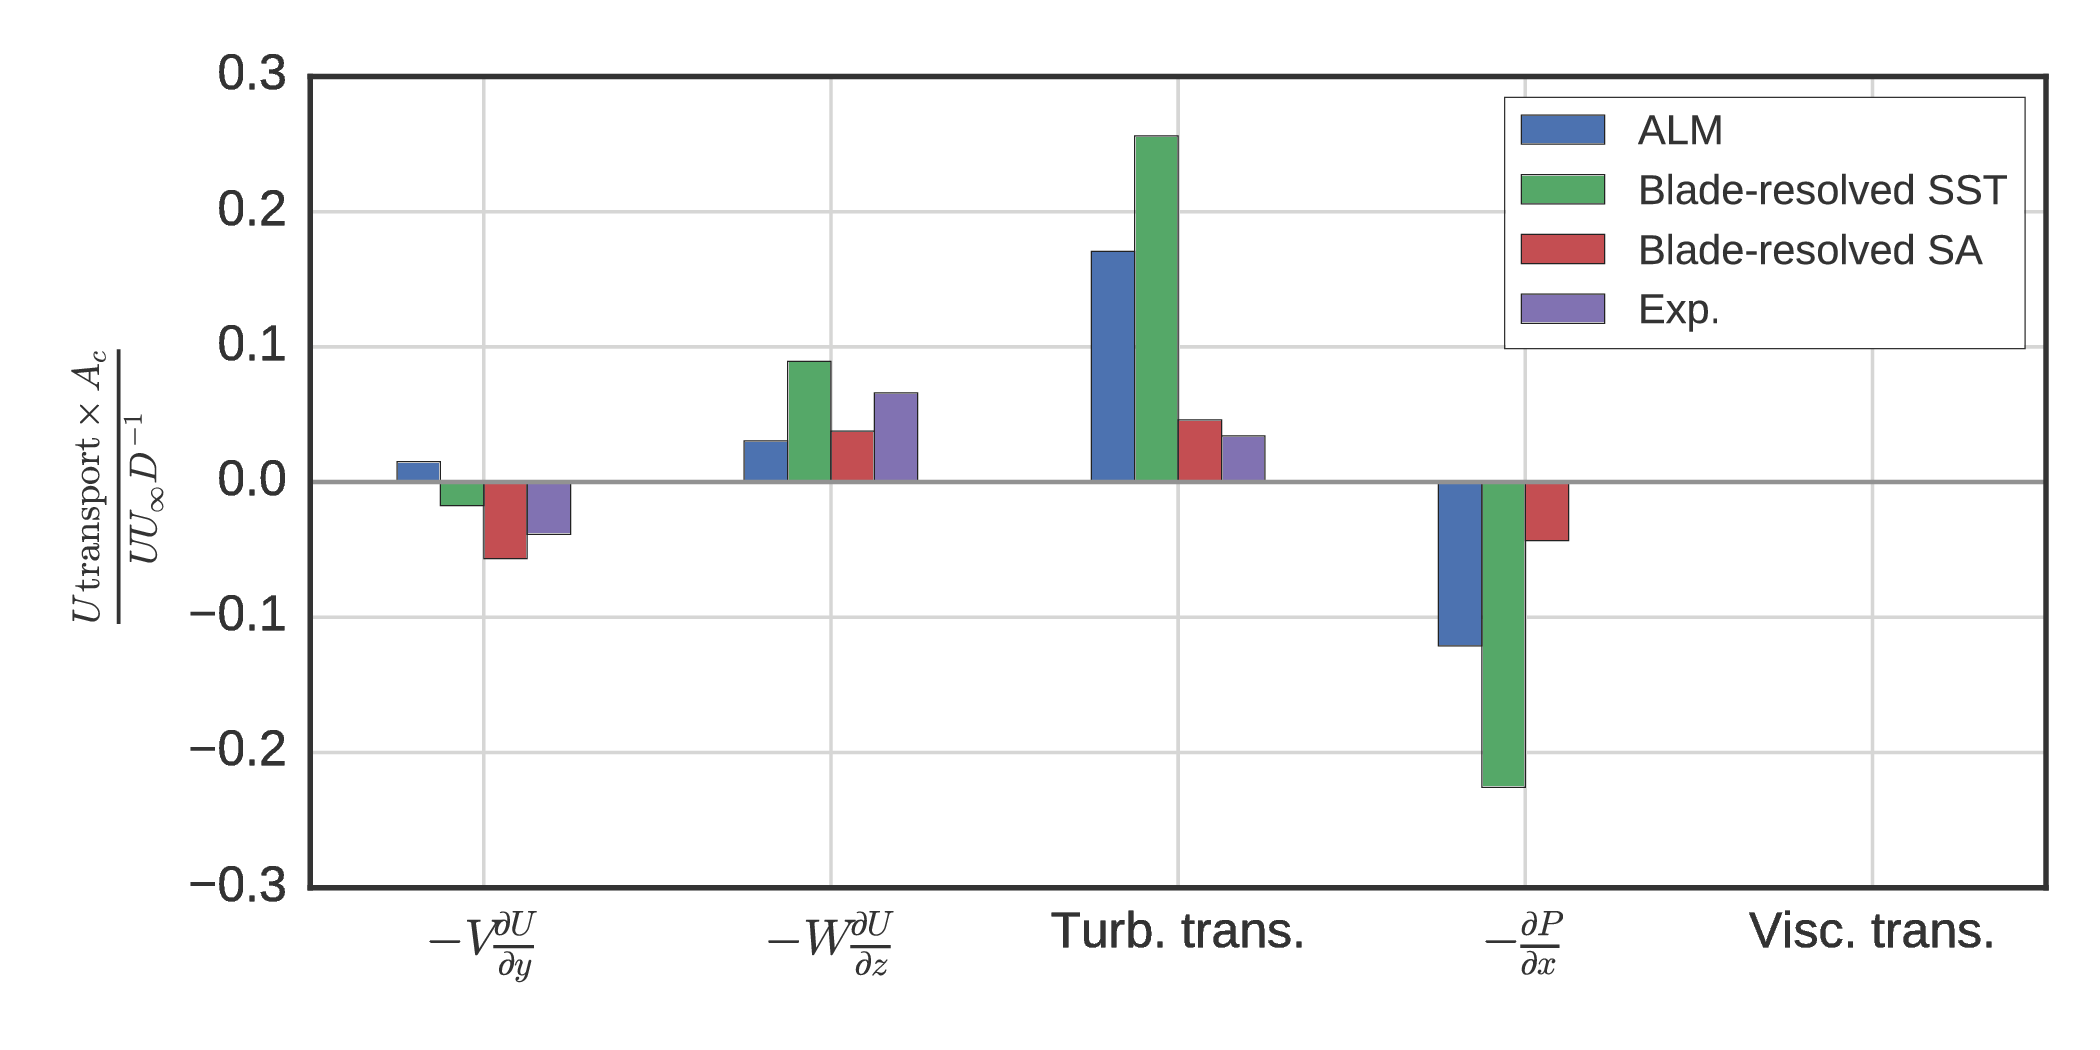
\includegraphics[width=0.85\textwidth]{RVAT-ALM_recovery-bar-chart}

    \caption{Weighted average momentum recovery terms for the UNH-RVAT actuator
        line model with a $k$--$\epsilon$ RANS closure, the two 3-D blade resolved
        RANS models described in Chapter~\ref{chap:CFD}, and the experiments in
        Chapter~\ref{chap:RVAT-baseline}}.
    
    \label{fig:RVAT-ALM-recovery}
\end{figure}


\subsection{RM2 RANS}

Figure~\ref{fig:RM2-ALM-perf-curves} shows the performance curves computed for
the RM2 by the ALM, and those from the tow tank experiments. As with the high
solidity RVAT, the drop in $C_P$ comes at higher $\lambda$.

\begin{figure}
    \centering
    
    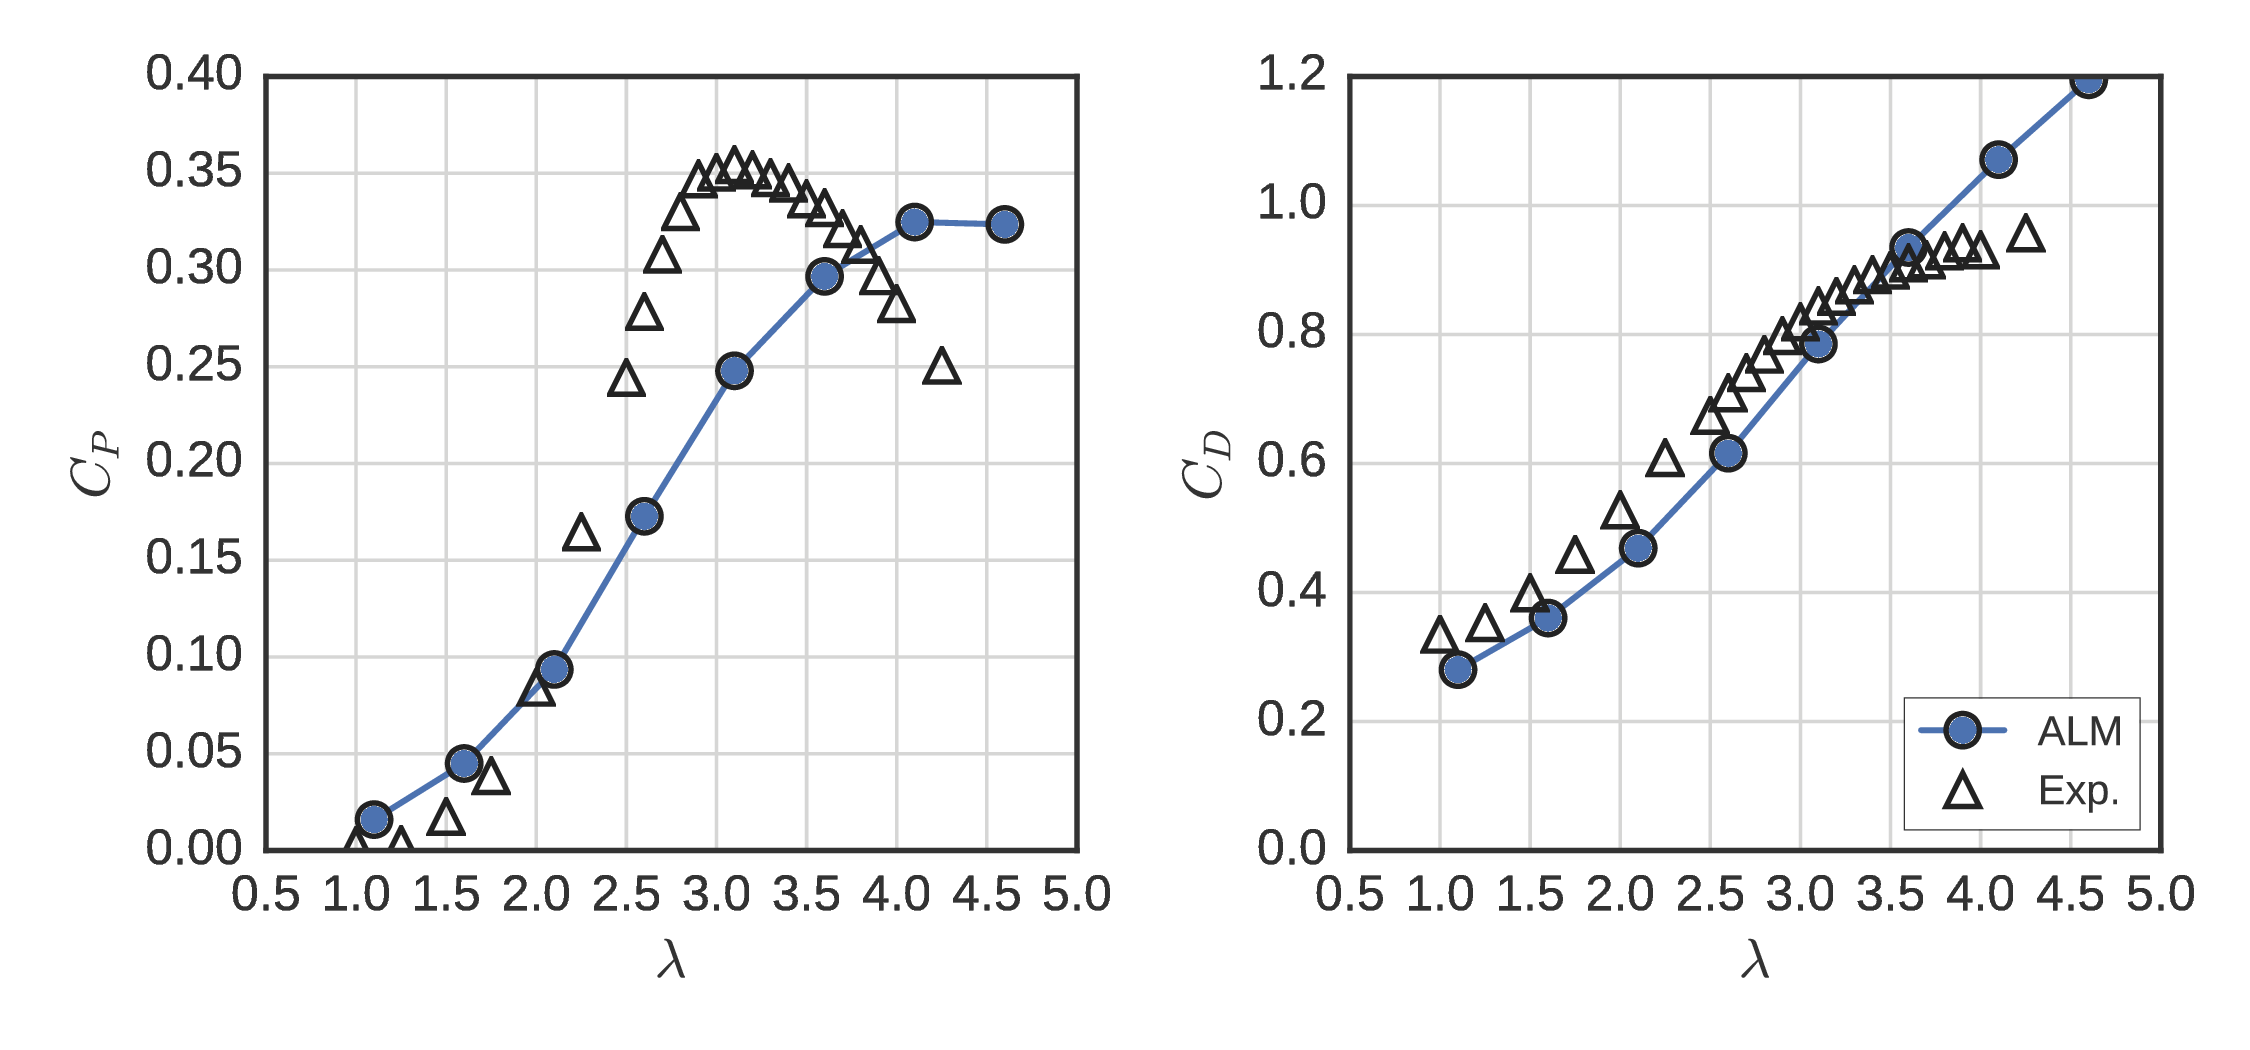
\includegraphics[width=0.85\textwidth]{RM2-ALM_perf-curves}
    
    \caption{Power and drag coefficient curves computed for the RM2 using the
        ALM.}
    
    \label{fig:RM2-ALM-perf-curves}
\end{figure}

Figure~\ref{fig:RM2-ALM-meancontquiv} shows the mean velocity field computed
by the ALM for the RM2.

\begin{figure}
    \centering
    
    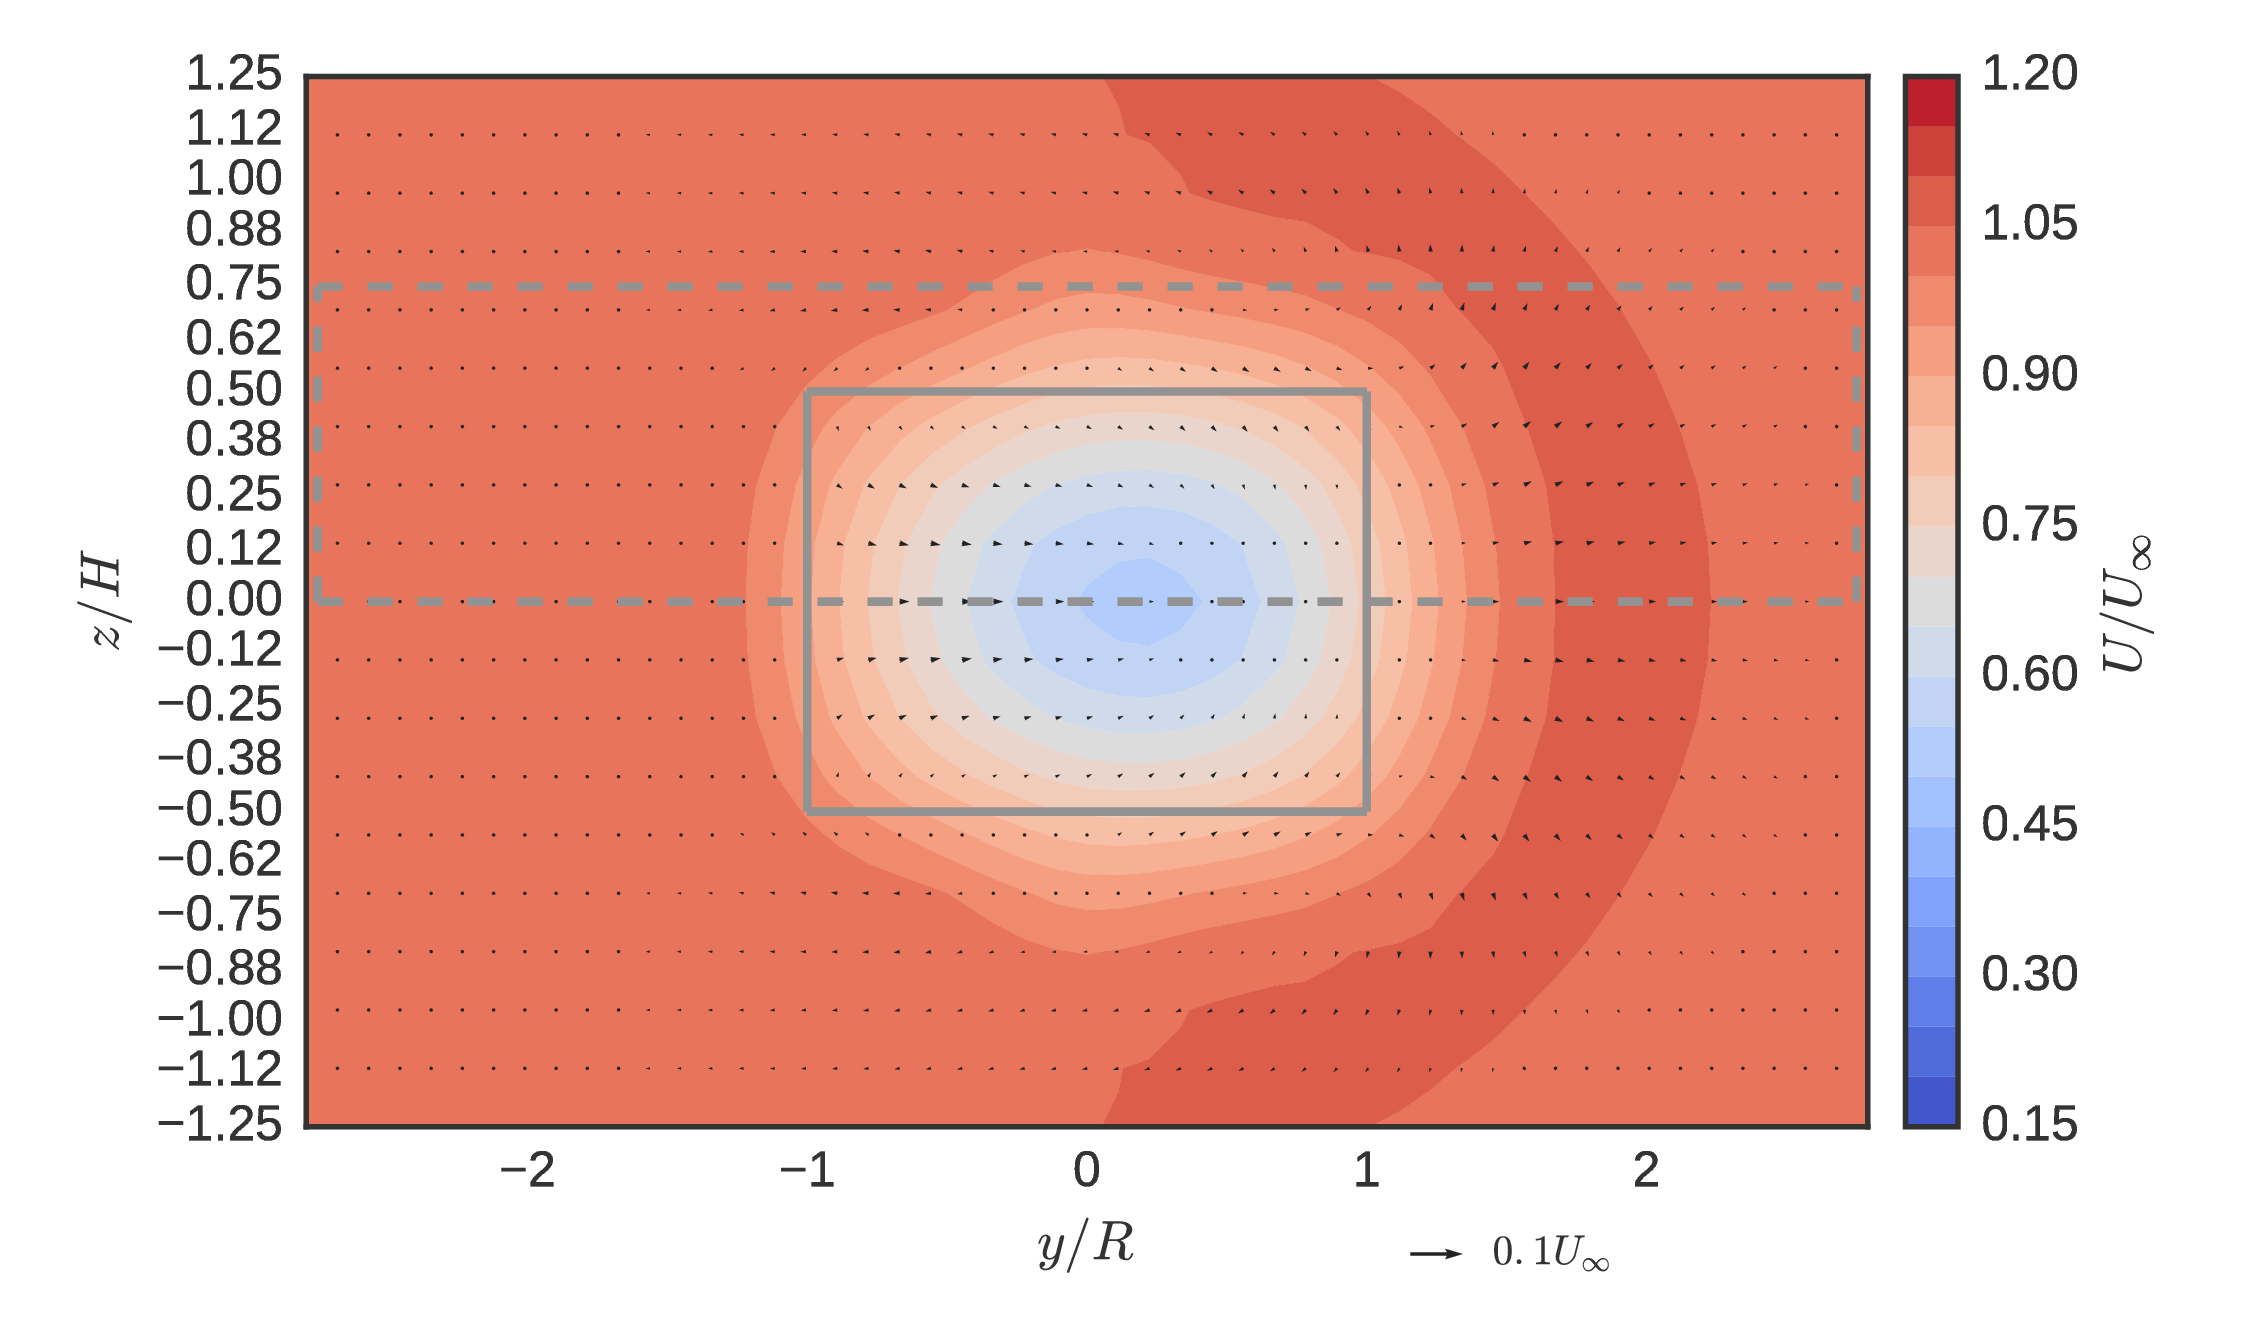
\includegraphics[width=0.9\textwidth]{RM2-ALM_meancontquiv}
    
    \caption{Mean velocity field at $x/D=0.93$ for the RM2 predicted by the
        ALM.}
    
    \label{fig:RM2-ALM-meancontquiv}
\end{figure}

Figure~\ref{fig:RM2-ALM-kcont} shows the ALM's turbulence kinetic energy
predictions in the near-wake of the RM2. Like for the UNH-RVAT, $k$ appears to
be concentrated on the $+y$ side of the rotor. However, overall levels of
turbulence are lower than for the UNH-RVAT, which is consistent with the
experimental results.

\begin{figure}
    \centering
    
    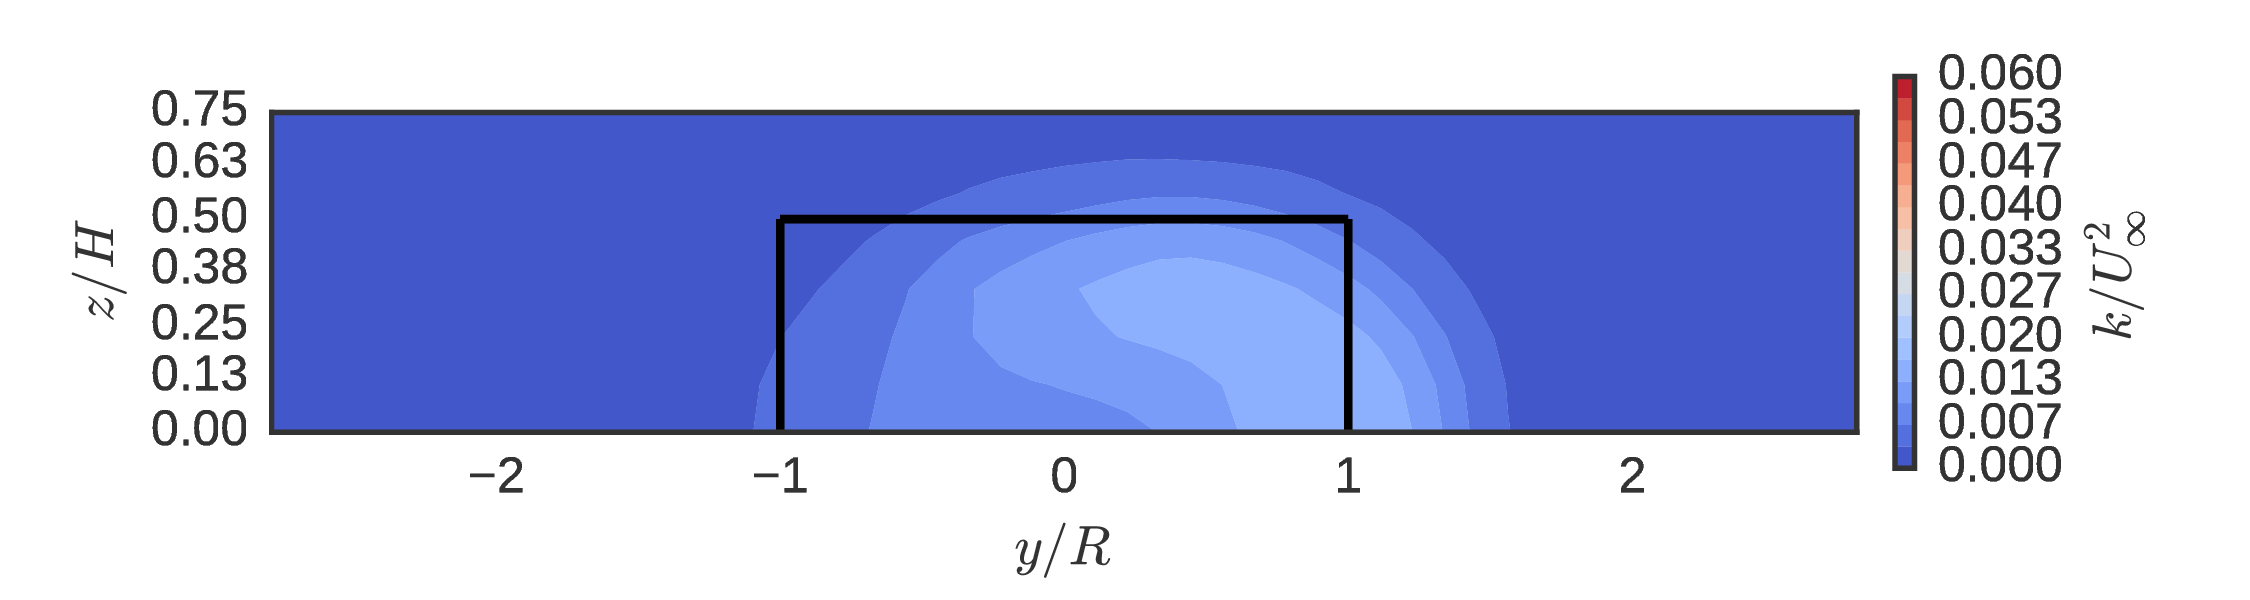
\includegraphics[width=0.9\textwidth]{RM2-ALM_kcont}
    
    \caption{Turbulence kinetic energy contours at $x/D=0.93$ behind the RM2
        predicted by the ALM.}
    
    \label{fig:RM2-ALM-kcont}
\end{figure}

\begin{figure}
    \centering
    
    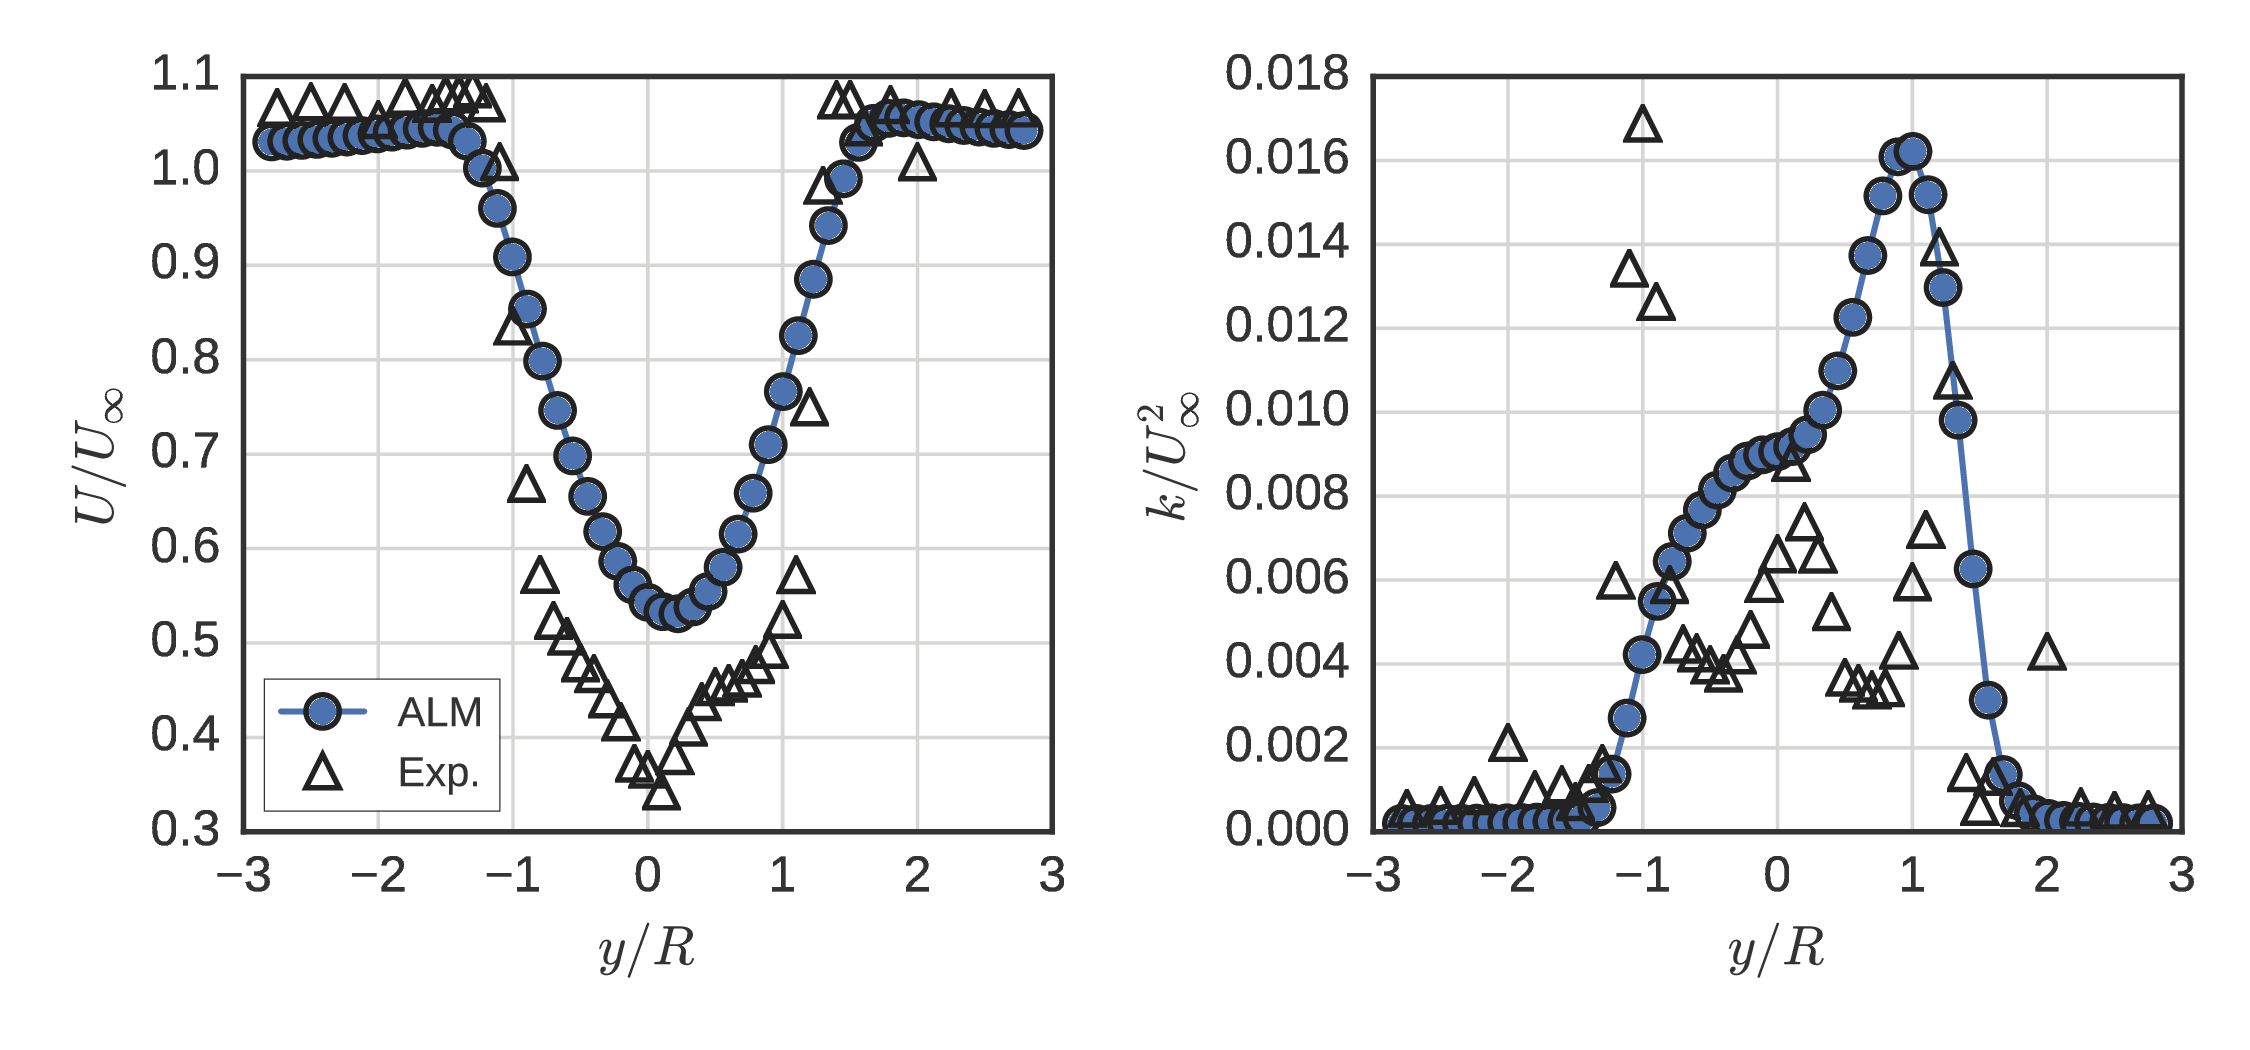
\includegraphics[width=0.85\textwidth]{RM2-ALM_wake-profiles}
    
    \caption{Mean streamwise velocity (left) and turbulence kinetic energy
        (right) profiles at $x/D=0.93$ and $z/H=0$ for the RM2 ALM.}
    
    \label{fig:RM2-ALM-profiles}
\end{figure}

\begin{figure}
    \centering
    
    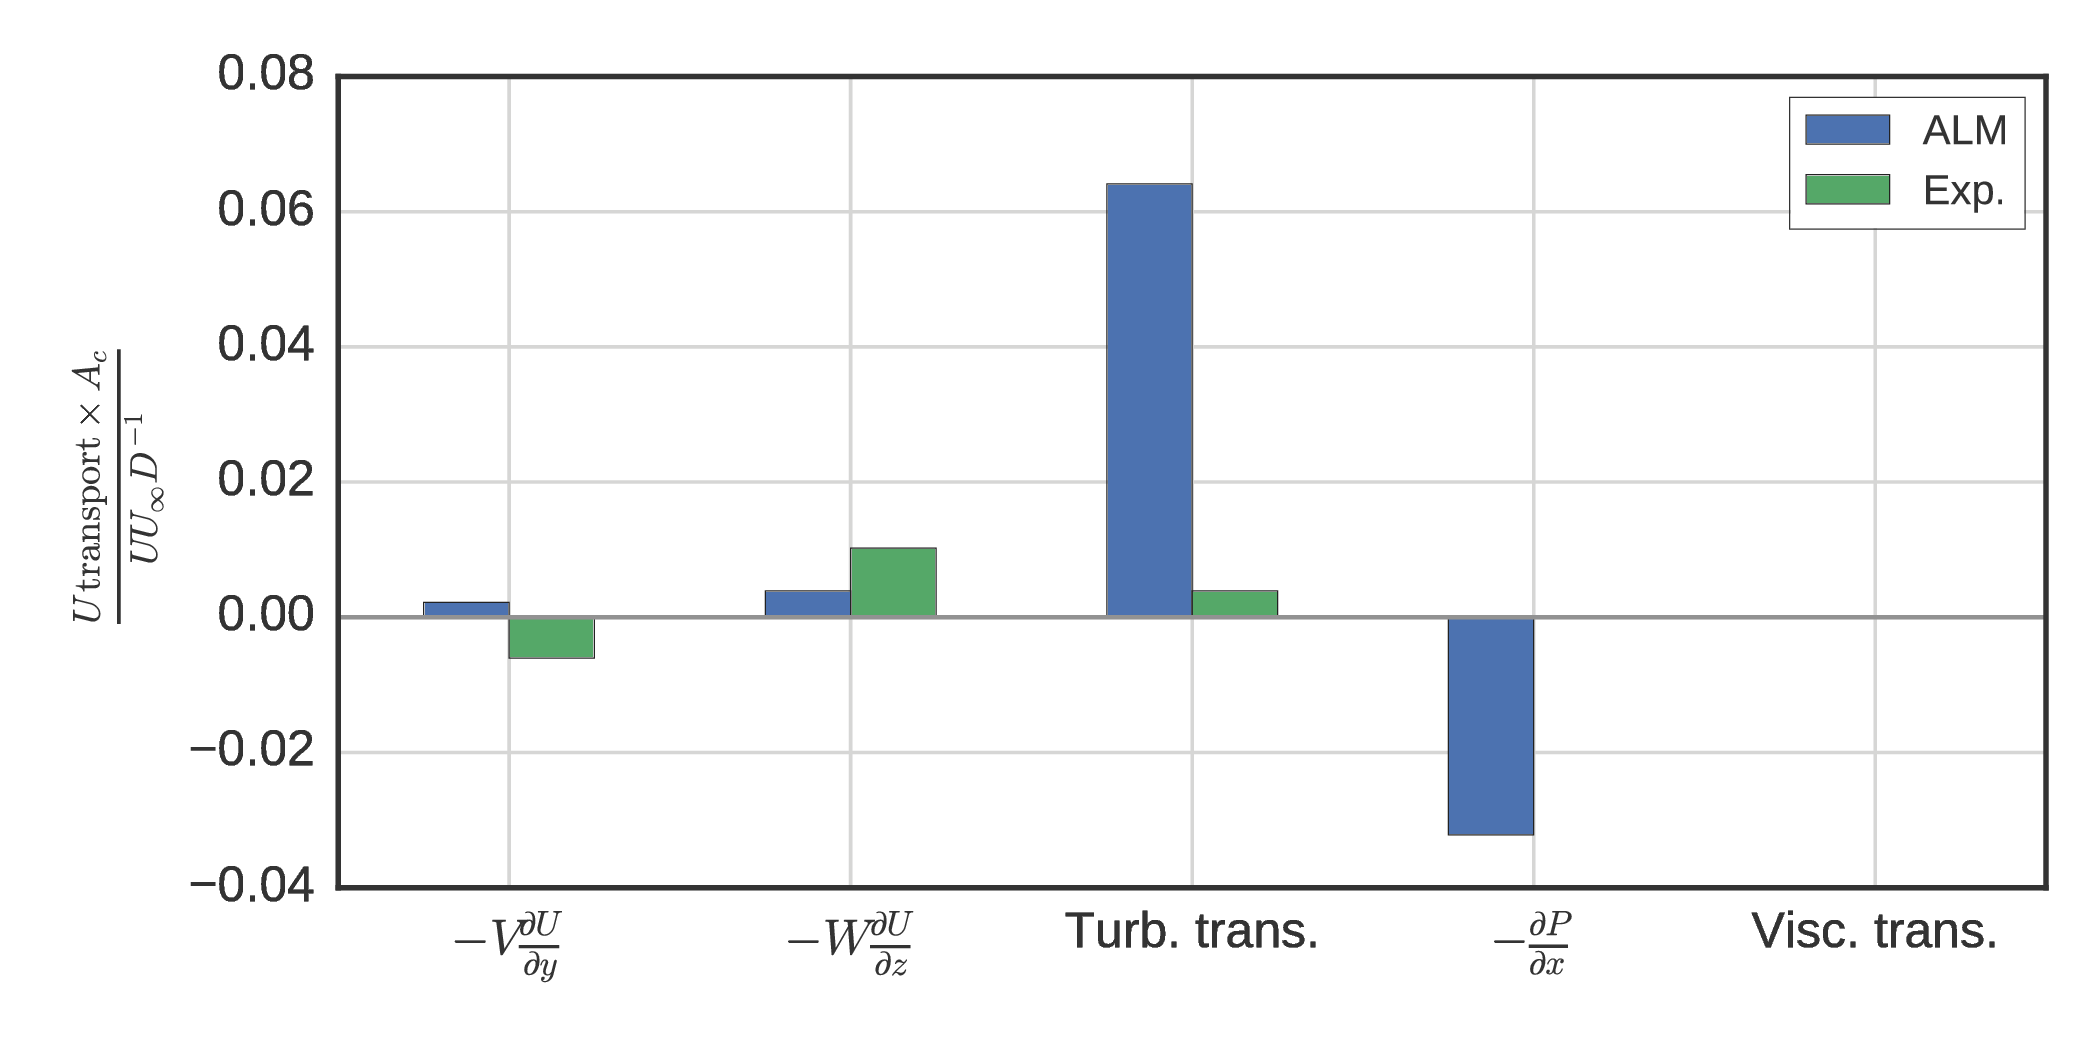
\includegraphics[width=0.85\textwidth]{RM2-ALM_recovery-bar-chart}
    
    \caption{Weighted average momentum recovery terms at $x/D=0.93$ for the RM2
        actuator line model with a $k$--$\epsilon$ RANS closure and the experiments
        described in Chapter~\ref{chap:RM2}}.
    
    \label{fig:RM2-ALM-recovery}
\end{figure}


\subsection{UNH-RVAT LES}

Since this was the most interesting wake structure...

Since the computational cost of LES is significantly higher than RANS,
verification was not performed. Instead, mesh resolution was chosen relative to
similar studies of turbine wake ALM. Of the studies surveyed
\cite{Shamsoddin2014,Archer2013,Martinez-Tossas2015a,Troldborg2007}, the mesh
resolution ranged from 18--64 points per turbine diameter. The mesh here was set
accordingly by using a 16 point per meter base mesh, and refining twice in a
region containing the turbine to produce a 64 point per turbine diameter/height
resolution. The solver was run with a 0.002 second time step, which is
significantly within the limit described by \cite{Martinez-Tossas2015}, where an
actuator line element may not pass through more than one cell per time step.

For the LES, the default Smagorinsky model coefficients were used. 

Thanks to the ALM's general implementation as a source term, we are not tied to
any specific turbulence model. This means that as turbulence modeling and
computational power advance, the ALM can continue to be used. As a look towards
the future prospect of simulating large CFT arrays in great detail, a single CFT
was placed in a large eddy simulation (LES). Turbine geometry was identical to
the UNH-RVAT case, but the domain was extended to look at wake evolution father
downstream.

\begin{figure}
    \caption{Snapshot of vorticity contours for the UNH-RVAT LES case.}
    
    \label{RVAT-LES}
\end{figure}

\todo[inline]{Add meancontquiv for RVAT LES case?}


The planar weighted sum of streamwise momentum recovery terms was computed in
the same was as for the RANS cases with the exception of the turbulent transport
term, which for the LES was computed from the $x$-component of the divergence of
the Reynolds stress tensor:
\begin{equation}
    \text{Turb. trans.} = -\frac{\partial}{\partial x_j}
    \overline{u^\prime u^\prime_j},
\end{equation}
where $U$ and $u$ (without subscripts) indicate streamwise components.

\todo[inline]{Add recovery terms for RVAT LES case?}


\section{Computational cost}

\todo[inline]{Move this section to conclusions or top-level results section like
    CFD chapter.}

Compared to blade-resolved RANS, the ALM can solve a standalone turbine case on
the order of CPU minutes per second of simulated time versus 1,000 CPU hours per
second---a savings of 4 orders of magnitude. However, the results for the ALM
are not quite as detailed. For example, the $-y$ tip vortex (where dynamic stall
is occurring) is not captured by the ALM.

The RANS simulations took "$O(0.1)$ CPU hours per second of simulated time,
while the LES took $O(10)$.


\section{Conclusions}

In this chapter the actuator line model has been developed and tested against
the cross-flow turbine validation datasets acquired in previous chapters.

Despite a small loss in accuracy, the ALM can do a reasonable job predicting the
performance and wake of a cross-flow turbine. It is therefore expected that this
tool will provide a much improved means of designing array layouts compared with
simple actuator disks, point sources, or superposition techniques---and all with
acceptable computational cost, i.e., not requiring HPC resources.

The ALM provides a more physical flow description compared to momentum and
vortex models, at a reasonable cost. The ALM has an important advantage over
vortex methods in that the computational expense is mainly due to solving the
flow field, which remains reasonably constant, where vortex methods increase in
computational complexity each time step. This is especially important for array
simulations, where for a given domain adding many turbines will be cheap in the
ALM compared to the rapidly increasing number of vortex elements generated by
each turbine. The ALM also drastically reduces computational effort compared to
blade-resolved CFD, while maintaining the unsteadiness of the wake not resolved
by a conventional actuator disk.

However, the mean flow structure and turbulence generation due to blade tip and
dynamic stall vortex shedding shows some discrepancy with experimental and
blade-resolved CFD. Extensions to the ALM to deal with these shortcomings should
be developed, e.g., a turbulence injection model as developed by James \emph{et
    al.} \cite{James2010} or a model that will ``turn'' the ALM body force vectors
to approach the effects of leading and trailing edge separation during dynamic
stall.

%%% Below from proposal introduction

If the proposed body force model is inadequate for postdicting our experimental
performance data, one possible strategy for improving accuracy is to generate
foil coefficient databases with more dimensions, e.g., blade pitch rate or local
turbulence levels. It may also be possible to modify the dynamic loading models
based on insight from the body-fitted grid simulations.

%%% End from proposal introduction

At the very least, the prospect of using ALM simulations to drive down
computational cost of RANS by nearly five orders of magnitude justifies further
development.

At contemporary levels of computing power, the ALM is a useful tool when HPC is
not feasible. Furthermore, if arrays of CFTs become make it to commercial scale,
the ALM combined with LES represents one of the highest fidelity tools
available.

From an engineering standpoint, the ALM was successful at ranking the two
turbines' performance. $\lambda_0$ was identified well for the UNH-RVAT, as well
as its maximum $C_P$. For the RM2, which was expected to be easier to model
thanks to its lower $c/R$ ratio, $C_{P_{\max}}$ was computed well, though
$\lambda_0$ was not. However, it may be desirable to operate the RM2 at slightly
higher $\lambda \approx 3.5$ to mitigate the fatigue loading due to stall, where
$C_P$ is close to $C_{P_{\max}}$, and the ALM was more successful.


\section{Future work}

Since the ALM relies on static foil coefficient data, it is crucial that more be
measured and published openly, to allow the exploration of new turbine designs.
There is some doubt regarding the veracity of the Sheldahl and Klimas NACA foil
data \cite{Bedon2014}. However, competing datasets at large laboratory scale
Reynolds numbers are rare, even for the standard symmetrical foils. CFD may play
a role in generating new data, but models must be rigorously validated, given
the difficulty in predicting stall and its importance on CFT blade loading.

The effects of local turbulence levels on foil coefficient data could be a model
worth developing, since stall delay could affect loading significantly.

The ALM should next be validated with far-wake data and/or data from two CFTs
operating in proximity of each other.

A better Reynolds number correction for foil data could be developed---one that
can successfully reshape the coefficient curves for the shifting stall point.

Rotor angular speed control via generator models could be included to test the
effectiveness of various control schemes, e.g., sinusoidal $\lambda$ set points,
which have been shown in some cases to improve mean power coefficient.
\todo[inline]{Get some information and a citation about UW's work on CFT
    controls.}

The ALM should be evaluated for its use in modeling CFT arrays.

The ALM and its associated loading models could be used to develop dynamic wall
functions for coarse blade-resolved RANS, which would provide yet another option
for reduced computational expense.

Flow curvature corrections should be examined in more detail, and it may be
beneficial to develop models to transform entire foil datasets to match their
virtual camber, as suggested by Migliore \emph{et al.}~\cite{Migliore1980}.

Since \textit{turbinesFoam} is compatible with OpenFOAM's volume of fluid (VOF)
multiphase flow solver \textit{interFoam}, the ALM's effectiveness should be
assessed for predicting the generation and interaction of turbines with surface
waves. The ADV positioning system developed in Chapter~\ref{chap:exp-setup}
could be retrofitted with a wave staff to measure and validate the free surface
disturbance, which could be key to predicting the effects of placing turbines in
channels at high blockage ratio.

The effects of separation at blade--strut attachment points should be further
studied. This may be one reason the turbine performance is overestimated at high
$\lambda$, since these effects scale approximately with
$\lambda^2$--$\lambda^3$.


\subsection{Turbulence injection}

Conventional blade element simulations use either momentum or vortex methods to
solve for the incident flow field, but these methods do not model the effects of
turbulence. With the actuator line model, there is the opportunity to improve
the physical realism by not only adding a source term to the momentum equation,
but also to the turbulence model equations. James \emph{et al.} \cite{James2010}
implemented an actuator disk model in a RANS model with a $k$--$\epsilon$
closure, which ``injected'' $k$ and $\epsilon$ from the actuator disks to more
realistically simulate the turbine's turbulent wake and enhance momentum
transport. However, to the author's knowledge injecting turbulence quantities
has never been done in an actuator line model.

The primary goal was to develop a simple model that use blade loading to compute
turbulence values to inject locally into the $k$--$\epsilon$ RANS model scalar
fields. Initial targets for local turbulence levels were established by
simulating a 2-D symmetrical NACA 0021 airfoil at $Re_c = 2 \times 10^5$ using
the $k$--$\omega$ SST turbulence model, given its favorable reputation for
predicting stall. The model results for the specific dissipation $\omega$ were
converted to $\epsilon$ by \cite{Wilcox1994}
\begin{equation}
    \epsilon = \beta^* \omega k.
\end{equation}

A snapshot of the mesh for the 2-D blade-resolved static foil case is shown in
Figure~\ref{fig:NACA-foil-mesh}. 30 seconds of unsteady flow over the foil were
simulated using OpenFOAM's \textit{pimpleFoam} solver and averages were
calculated over the final 20 seconds. Mean turbulence quantities were sampled
along a vertical line at one chord length behind the quarter chord, and the
maximum turbulence scalar value was stored. The goal here was not necessarily to
find injection rates that would correspond to experiments, but rather those that
would occur in a blade-resolved RANS case, though our results from
Chapter~\ref{chap:CFD} indicate that for the $k$--$\omega$ RANS model these may
be equivalent.

\begin{figure}
    \centering
    
    \caption{2-D NACA 0021 foil mesh at 20 degrees angle of attack.}
    
    \label{fig:NACA-foil-mesh}
\end{figure}

Mean turbulence kinetic energy contours next to the foil are shown in
Figure~\ref{fig:NACA-foil-k} and the foil force coefficients and sampled mean
turbulence values are shown in Figure~\ref{fig:NACA-foil-coeffs}. There is a
clear correlation between drag and turbulence in the foil wake, though
turbulence levels seem to saturate around the static stall angle. These features
motivated the development of a simple linear model for turbulence injection rate
as a function of drag coefficient.

\begin{figure}
    \centering
    
    \caption{Mean turbulence kinetic energy computed around the 2-D NACA 0021
        foil at 20 degrees angle of attack.}
    
    \label{fig:NACA-foil-k}
\end{figure}

\begin{figure}
    \centering
    
    \caption{Simulated force coefficients and turbulence quantities plotted
        versus angle of attack for a 2-D NACA 0021.}
    
    \label{fig:NACA-foil-coeffs}
\end{figure}

Turbulence kinetic energy was regressed linearly against the drag coefficient up
to the static stall angle, which was determined numerically as the angle of
attack at which $C_d$ first increased at more than 0.02 per degree. For angles
above static stall, the average value of $k$ was taken to be the limit for
turbulence injection. The turbulent dissipation $\epsilon$ was regressed
linearly against $k^{3/2}$, which was motivated by the relationship from the
standard $k$--$\epsilon$ model \cite{Wilcox1994}:
\begin{equation}
    \epsilon = C_\mu \frac{k^{3/2}}{l},
\end{equation}
where $C_\mu$ is a closure coefficient, typically 0.09.

Figure~\ref{fig:NACA-foil-fits} shows the simulation results plotted along with
their associated fit lines. The regressions and their resulting parameters
inspired injection rates for $k$ and $\epsilon$ of the form
\begin{equation}
    k_s = C_k \frac{U^3}{c} \min \left[ k_{\max} ,\, | m_k C_d +
    b_k | \right],
\end{equation}
and
\begin{equation}
    \epsilon_s = C_\epsilon \frac{k_s^{3/2}}{c},
\end{equation}
respectively, where $C_k$ and $C_\epsilon$ are tuning constants, $U$ is the
relative velocity magnitude, $c$ is the actuator line element chord length, and
$m_k$ and $b_k$ are the slope and intercept of the $k$ versus $C_d$ regression.

\begin{figure}
    \centering 
    
    \caption{Simulation results and linear regression models plotted for the 2-D
        NACA 0021 blade-resolved CFD simulation.}
    
    \label{fig:NACA-foil-fits}
\end{figure}

In practice, the model injection rate coefficients were tuned by trial-and-error
to fit the turbulence kinetic energy contours measured in the experiment. From
this perspective, the blade-resolved static foil modeling served to help
identify scaling relationships, but was not used to determine the coefficients
used in the ALM.
